\documentclass[10pt,a4paper]{article}

\usepackage[a4paper,margin=12mm]{geometry}
\usepackage{graphicx}
\usepackage{float}
\usepackage{amsmath}
\usepackage{booktabs}
\usepackage{array}
\usepackage{caption}
\usepackage{subcaption}
\usepackage{hyperref}

\hypersetup{colorlinks=true,linkcolor=black,urlcolor=blue}
\setlength{\parindent}{0pt}
\setlength{\parskip}{2pt}
\setlength{\tabcolsep}{4pt}
\renewcommand{\arraystretch}{1.06}
\captionsetup{font=footnotesize,skip=2pt}
\setlength{\textfloatsep}{6pt plus 1pt minus 1pt}
\setlength{\floatsep}{5pt plus 1pt minus 1pt}
\setlength{\intextsep}{5pt plus 1pt minus 1pt}
\setlength{\abovedisplayskip}{5pt plus 1pt minus 1pt}
\setlength{\belowdisplayskip}{5pt plus 1pt minus 1pt}
\sloppy
\graphicspath{{../}}

\begin{document}

\begin{center}
{\Large\bfseries Modularbeit FEM und CFD}\\
{\large Aufgabe 1 und Aufgabe 2, Projekt Nr. 27}\\
\vspace{0.5mm}
\begin{tabular}{ll}
CFD & ANSYS Fluent / PyFluent\\
Struktur & ANSYS MAPDL / Workbench, Python-FEM\\
\end{tabular}
\end{center}

\section*{Ausgangsdaten und Lastkette}
Für Projekt 27 gelten \(b=0.45\,\mathrm{m}\), \(h=0.25\,\mathrm{m}\), \(h_T=1.00\,\mathrm{m}\), \(c_\mathrm{Wind}=110\,\mathrm{km/h}=30.56\,\mathrm{m/s}\). Die Aluminiumtafel ist \(3.0\,\mathrm{m}\times2.0\,\mathrm{m}\times3\,\mathrm{mm}\) groß. Mit \(\rho=1.225\,\mathrm{kg/m^3}\) folgt
\[
q=\frac12\rho v^2=571.86\,\mathrm{Pa}.
\]
\begin{table}[H]\centering\small
\begin{tabular}{p{0.25\linewidth}p{0.29\linewidth}p{0.36\linewidth}}
\toprule
Teil & Ergebnisgröße & Verwendung im nächsten Schritt\\
\midrule
CFD & Windkraft \(F_D\), Druckverteilung & Flächenlast auf der Tafel\\
Schalenmodell Tafel & Spannungen, Verformungen, Lagerreaktionen & Bewertung der Lageridealisierung\\
Fachwerkmodell & Normalkräfte in Stäben & Dimensionierung der Stahlrohre\\
Python-FEM & Eigenes Stabwerksprogramm & Kontrolle der ANSYS-Stabwerkslösung\\
Aufgabe 2 & Kerbformzahl \(\alpha_k\) & unabhängige FEM-Aufgabe zur Lochscheibe\\
\bottomrule
\end{tabular}
\end{table}

\section{Aufgabe 1.1: Fluidmechanische Berechnung}

\subsection*{1.1 a) Geometrie und Netz}
Für die Strömungsrechnung wurde nur die Schildtafel modelliert; das Fachwerk trägt im Vergleich zur großen Schildfläche nur wenig zum Druckwiderstand bei. Die Rechendomäne reicht von \(x=-10\,\mathrm{m}\) bis \(x=30\,\mathrm{m}\), oben und unten bis \(y=\pm10\,\mathrm{m}\). Die Platte liegt bei \(x=\pm0.0015\,\mathrm{m}\), \(y=\pm1\,\mathrm{m}\). Die Netzverfeinerung liegt in den Bereichen hoher Gradienten:
\begin{itemize}
\item an der Vorderkante wegen Staudruck und Drucksprung,
\item an Ober- und Unterkante wegen Ablösung und Scherschichten,
\item im Nachlauf, weil dort Unterdruck und reduzierte Geschwindigkeit entstehen.
\end{itemize}

\subsection*{1.1 b) Randbedingungen und Löser}
\begin{table}[H]\centering\small
\begin{tabular}{lll}
\toprule
Rand & Bedingung & Begründung\\
\midrule
Einlass & \(v=30.56\,\mathrm{m/s}\) & Windgeschwindigkeit aus Projekt Nr. 27\\
Auslass & \(p=0\,\mathrm{Pa}\) relativ & freier Druckauslass\\
oben/unten & Symmetrie & freie Umgebung ohne Wandreibung\\
Schild & No-Slip-Wand & stationäre feste Oberfläche\\
\bottomrule
\end{tabular}
\end{table}

Als Turbulenzmodell wurde \(k\)-\(\omega\) SST verwendet, da es wandnahe Bereiche und Ablösung gut abbildet. Die stationäre SIMPLE-Rechnung lief über 500 Iterationen; die Residuen waren ab etwa Iteration 140 konvergiert, der Kraftmonitor ab etwa Iteration 80 stabil.

\begin{figure}[H]
\centering
\begin{subfigure}{0.49\linewidth}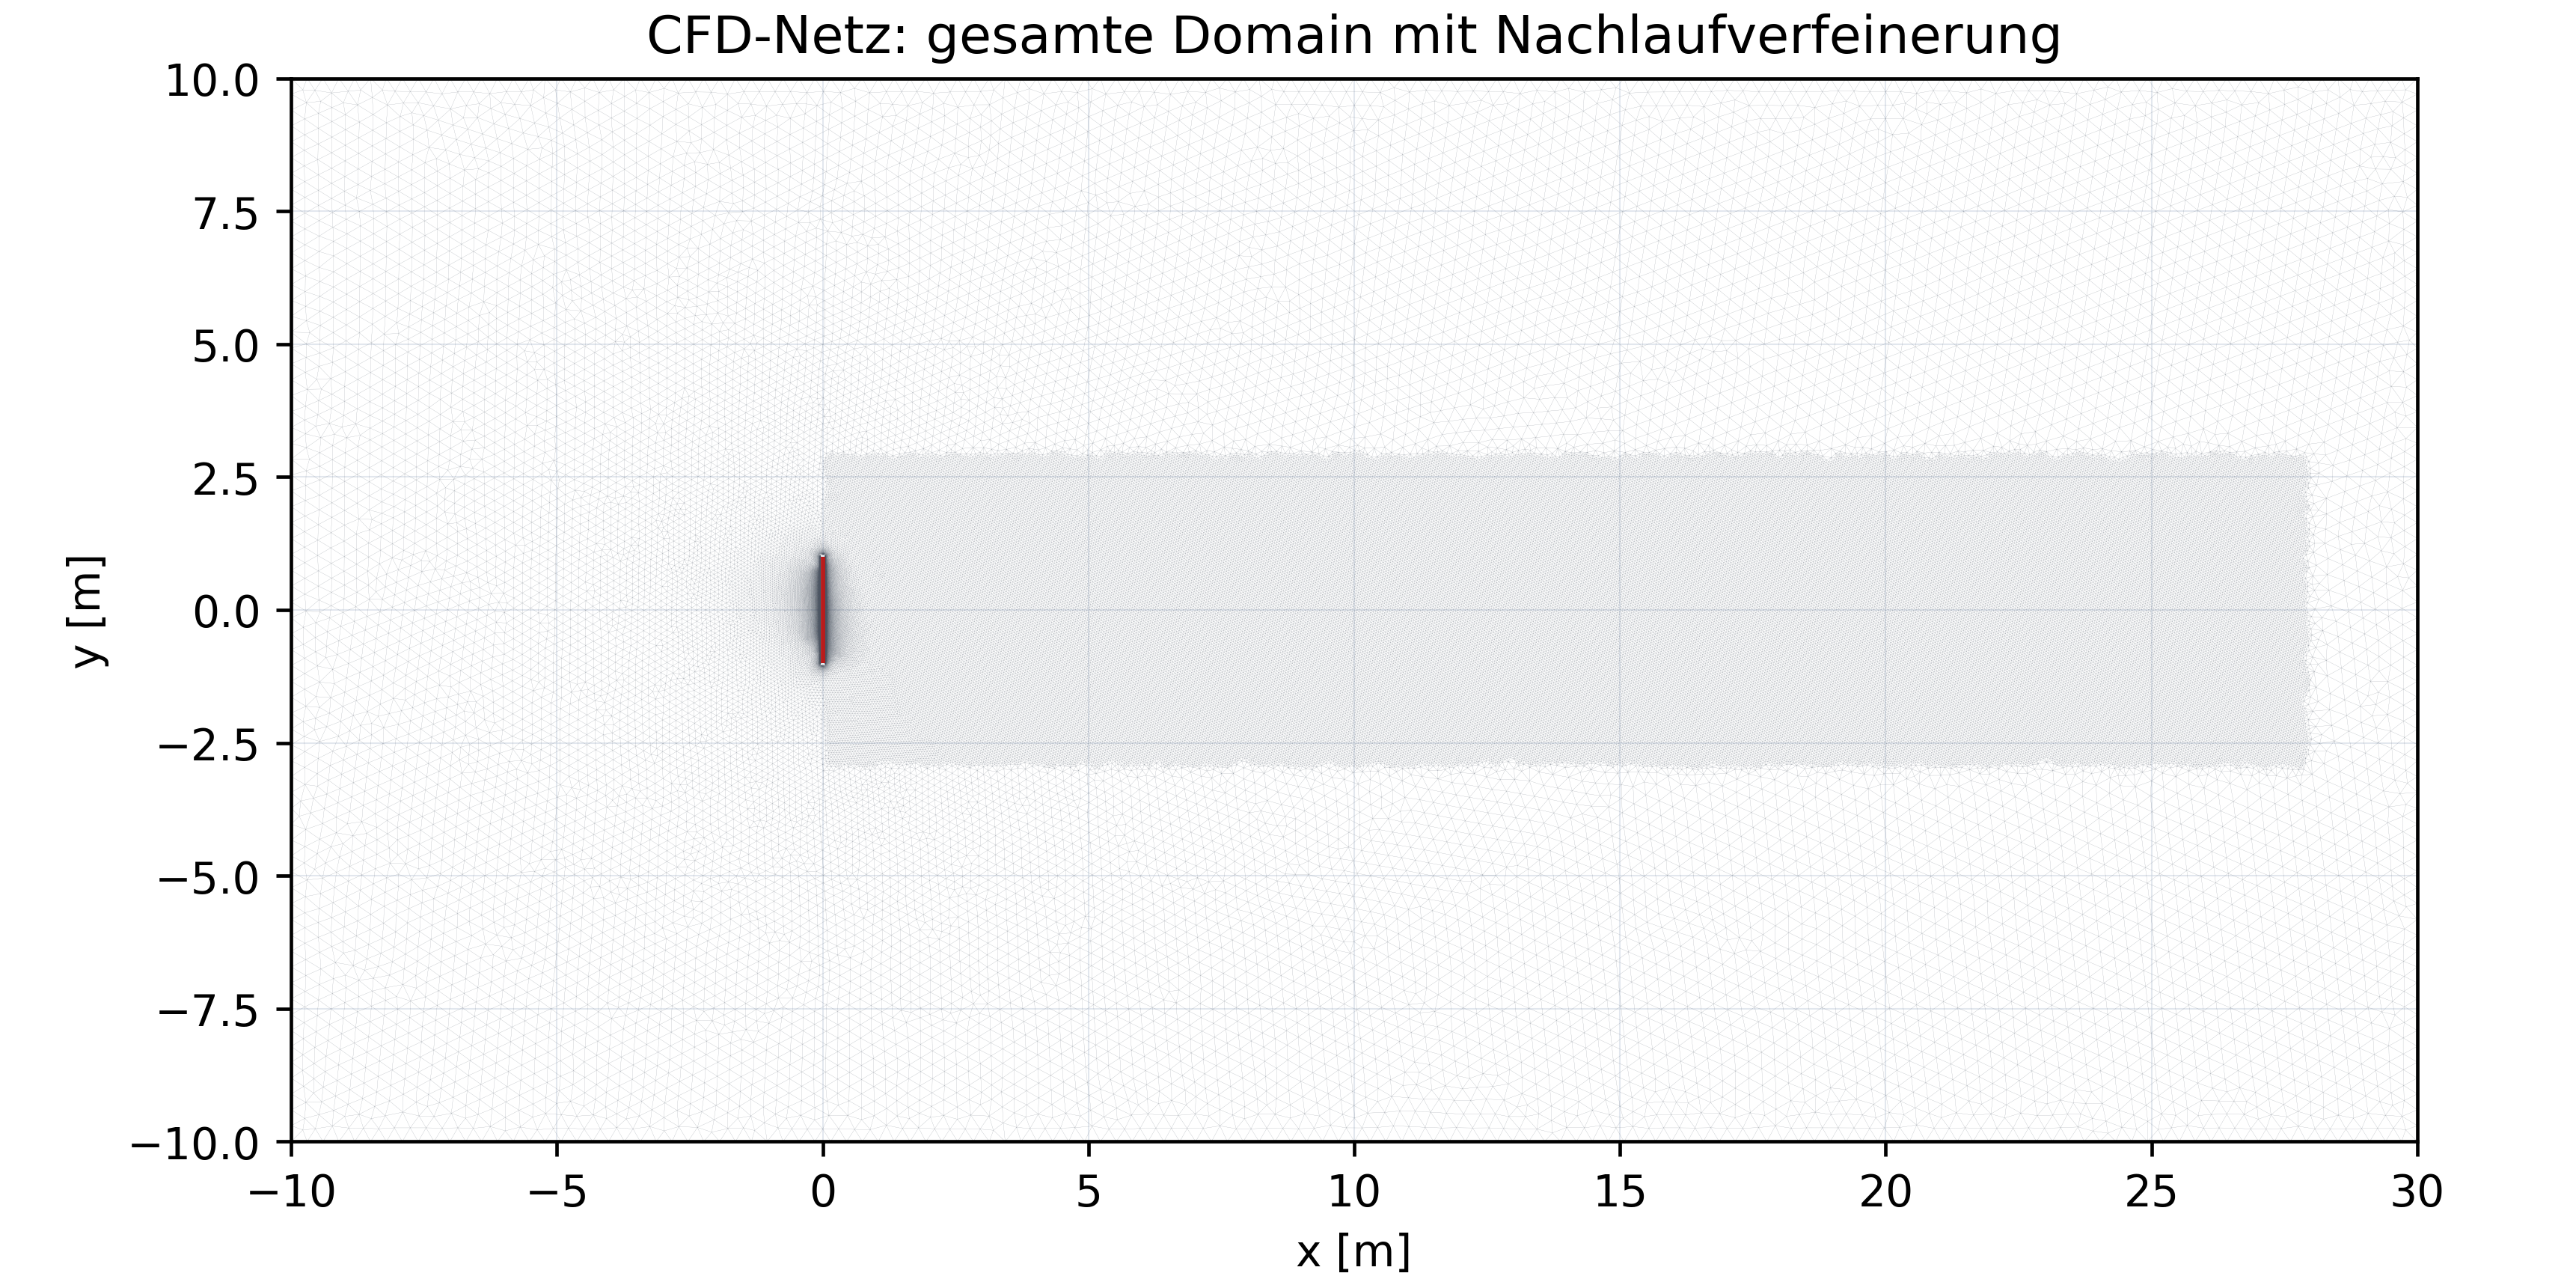
\includegraphics[width=\linewidth]{Aufgabe1/figures/mesh_overview_report.png}\caption{Gesamtes CFD-Netz}\end{subfigure}
\begin{subfigure}{0.49\linewidth}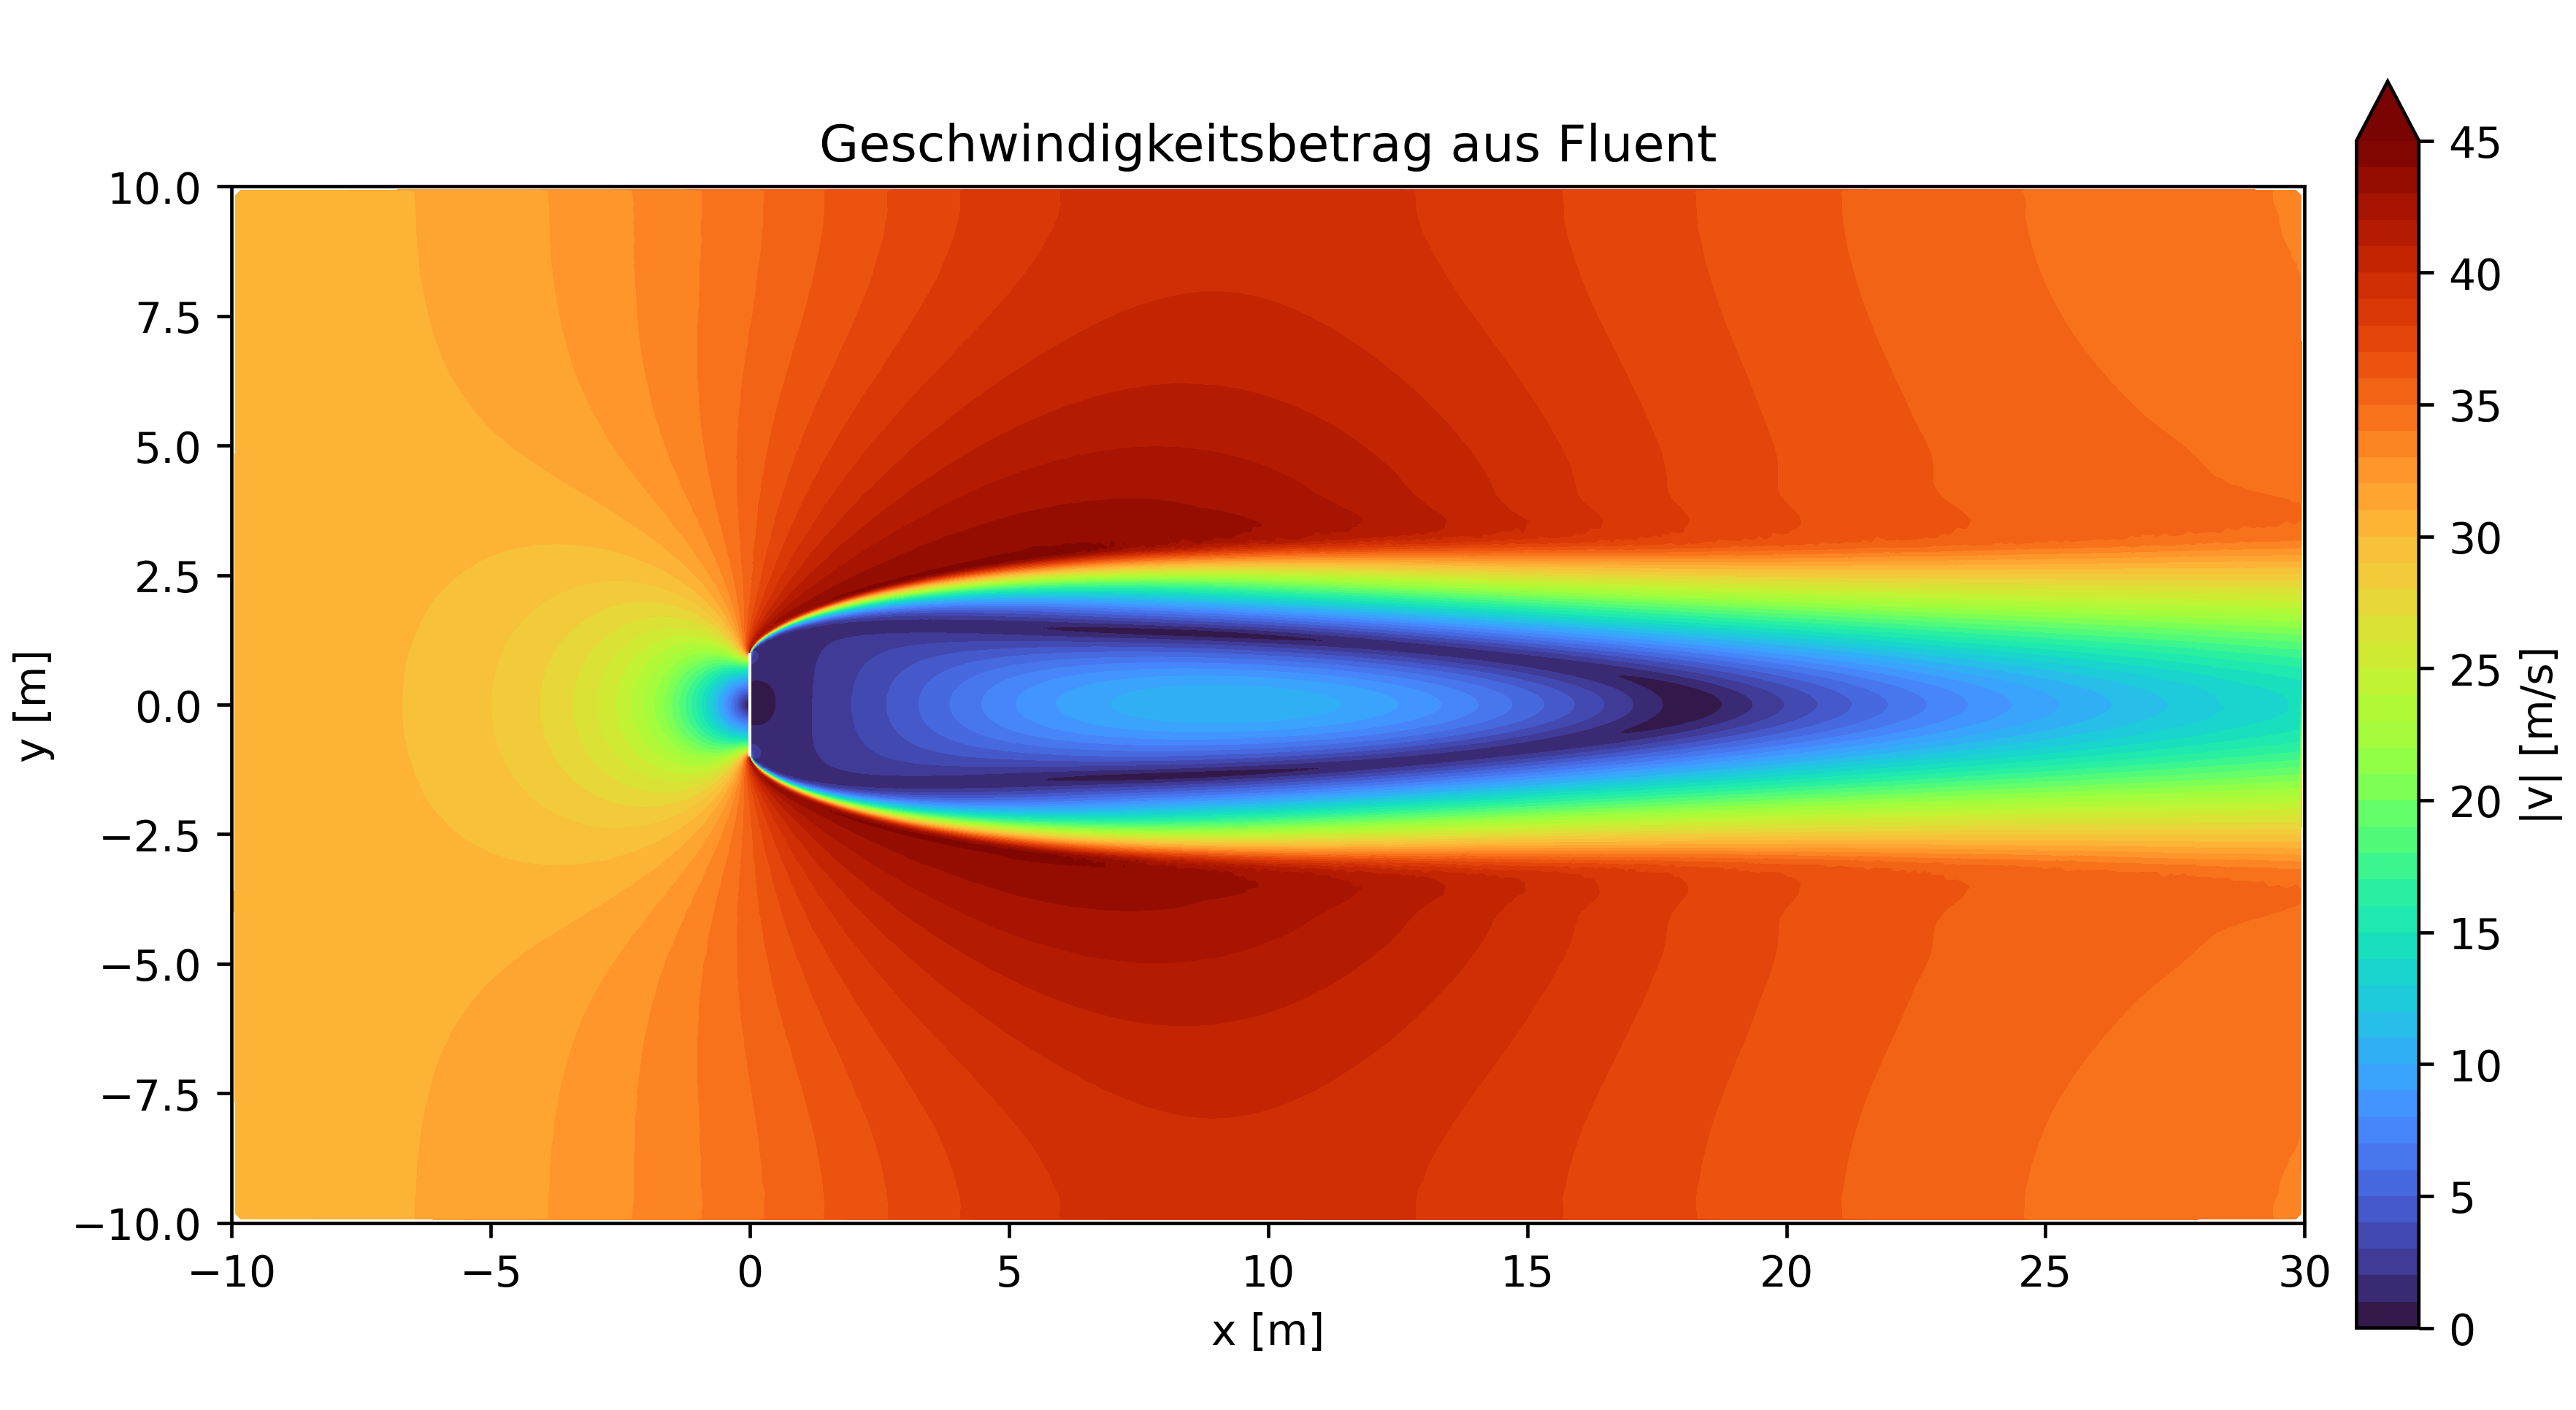
\includegraphics[width=\linewidth]{Aufgabe1/figures/contour_velocity_report.png}\caption{Geschwindigkeitsfeld}\end{subfigure}
\end{figure}

\subsection*{1.1 c)--d) Strömungsbild, Druckverteilung und Kontrolle}
Das Strömungsbild entspricht der Erwartung für eine quer angeströmte ebene Platte: vor dem Schild entsteht ein Staugebiet mit hohem Druck; an den scharfen Kanten löst die Strömung ab; hinter dem Schild bildet sich ein breiter Nachlauf mit Unterdruck und kleiner Geschwindigkeit. Der Kraftbeitrag kommt deshalb fast vollständig aus der Druckdifferenz zwischen Vorder- und Rückseite.

\begin{figure}[H]
\centering
\begin{subfigure}{0.49\linewidth}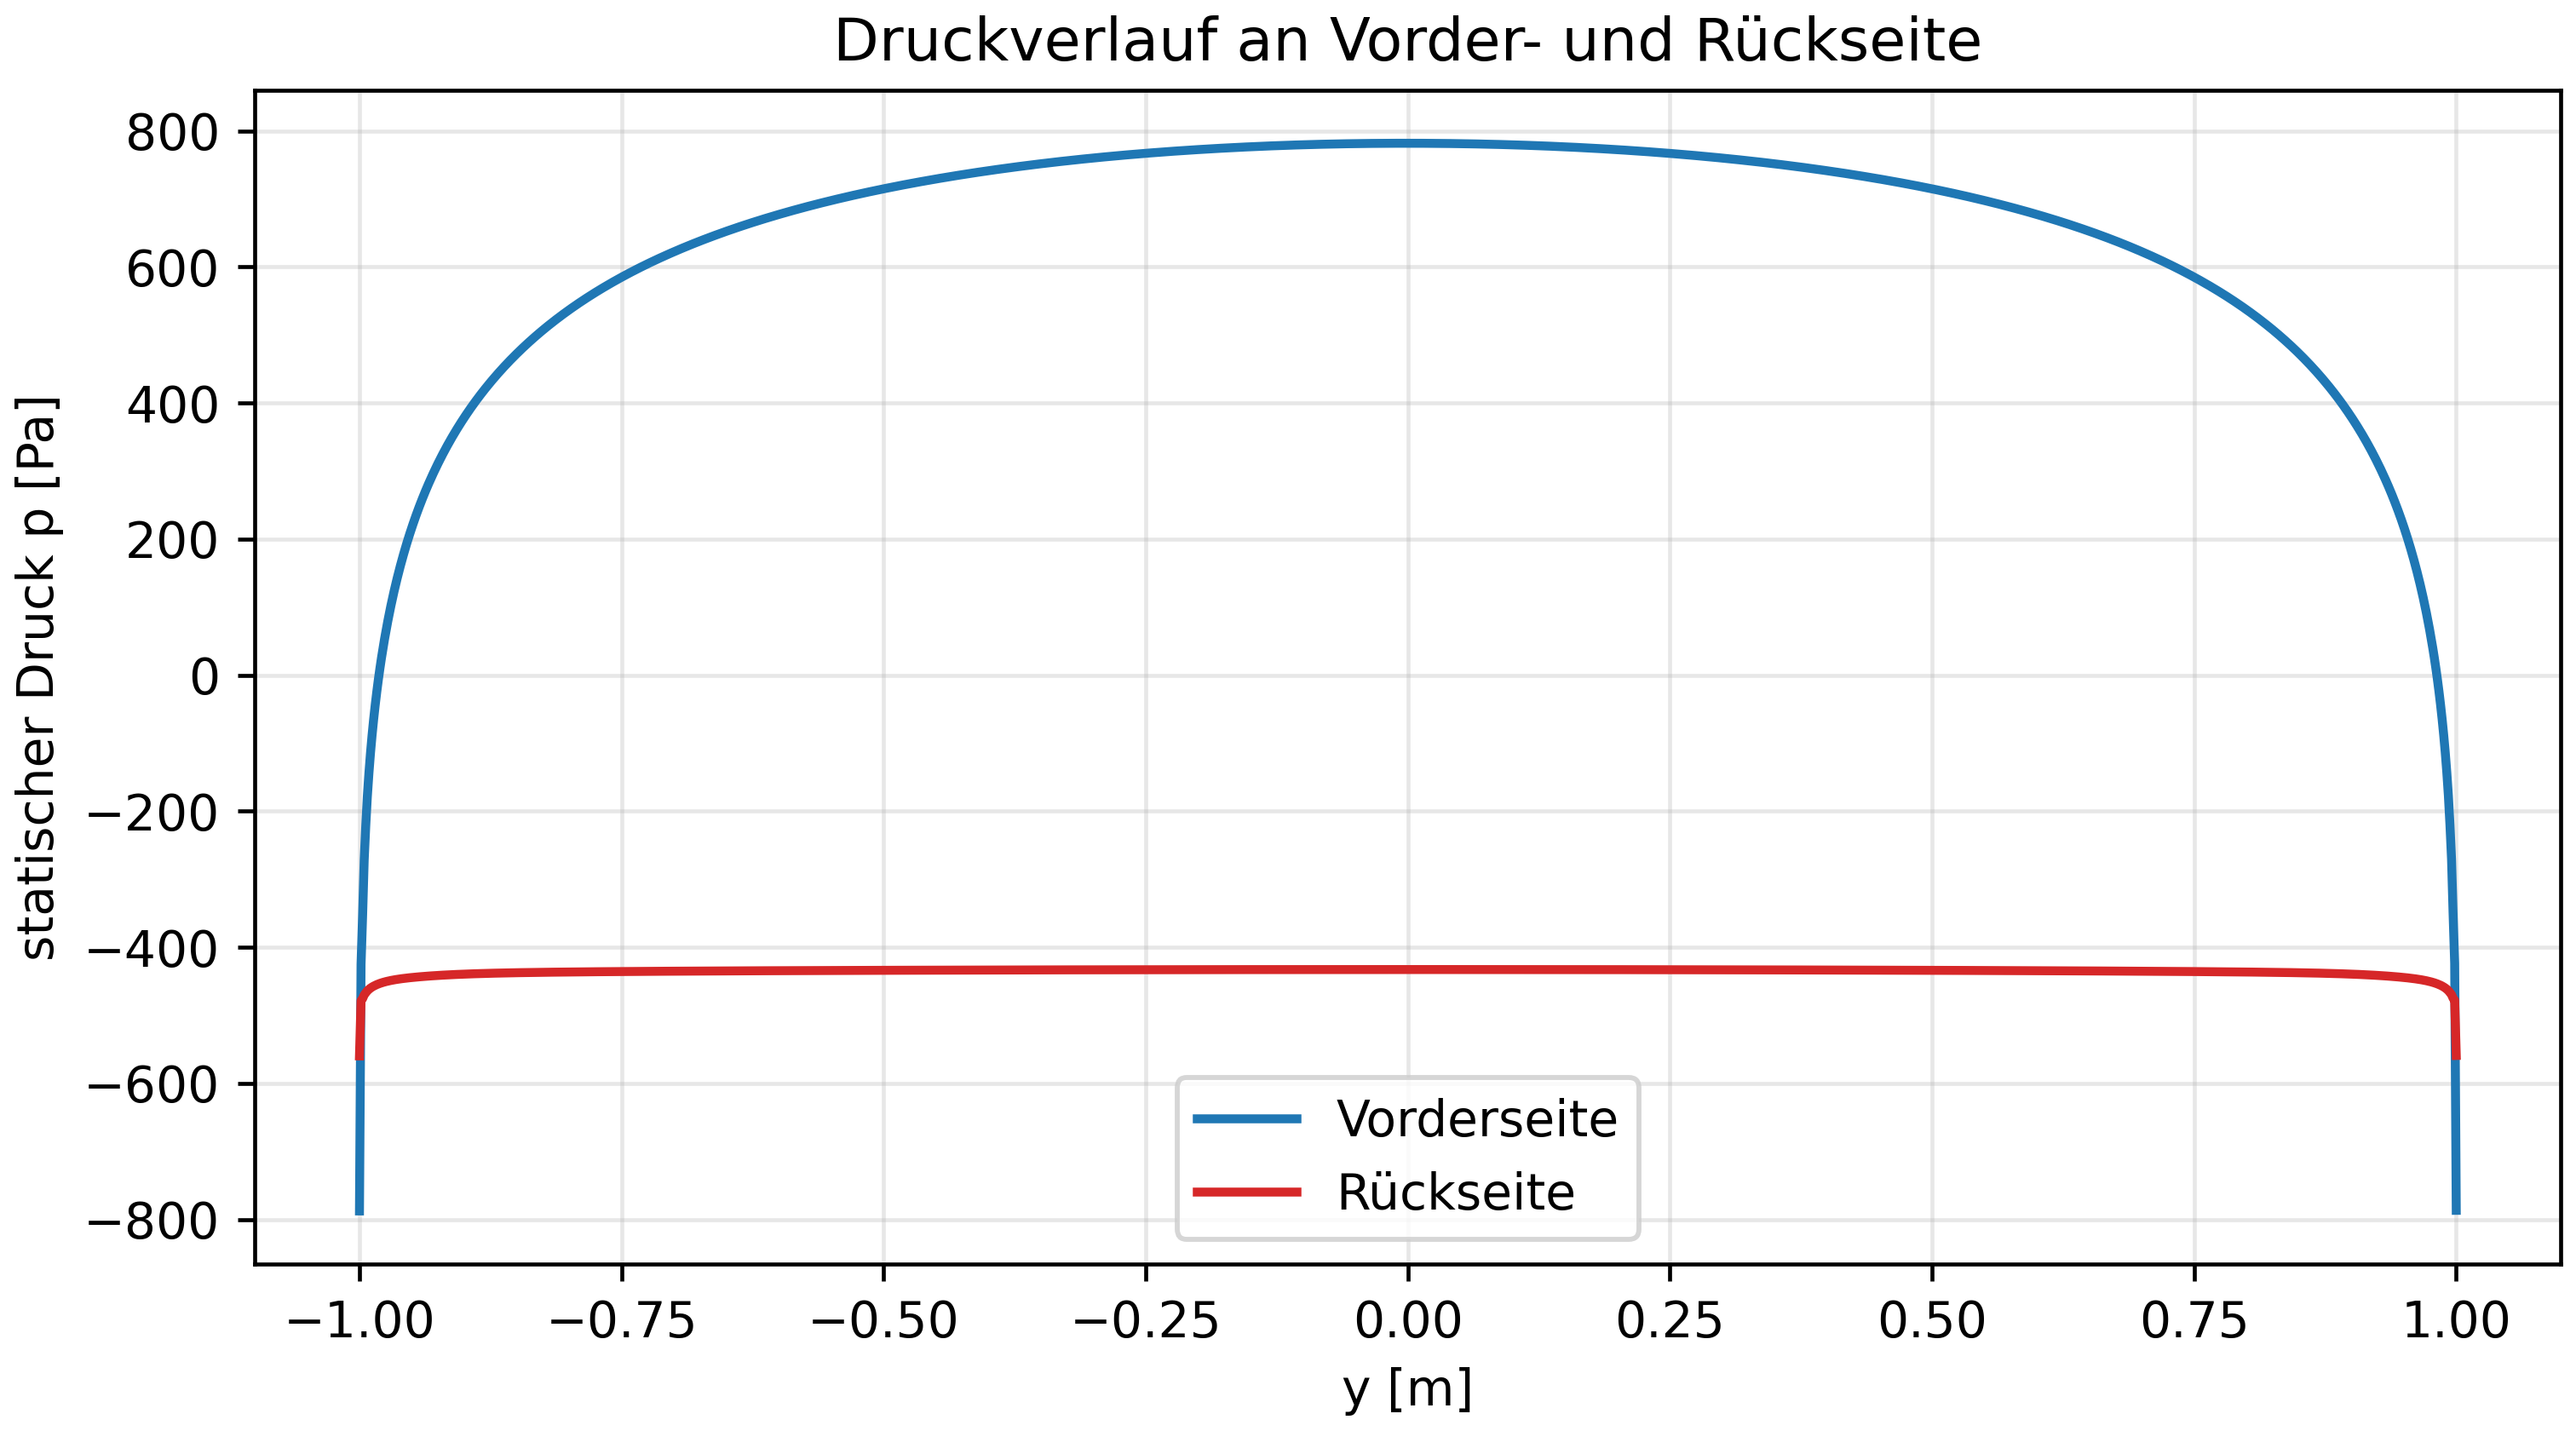
\includegraphics[width=\linewidth]{Aufgabe1/figures/pressure_distribution.png}\caption{Druckverlauf}\end{subfigure}
\begin{subfigure}{0.49\linewidth}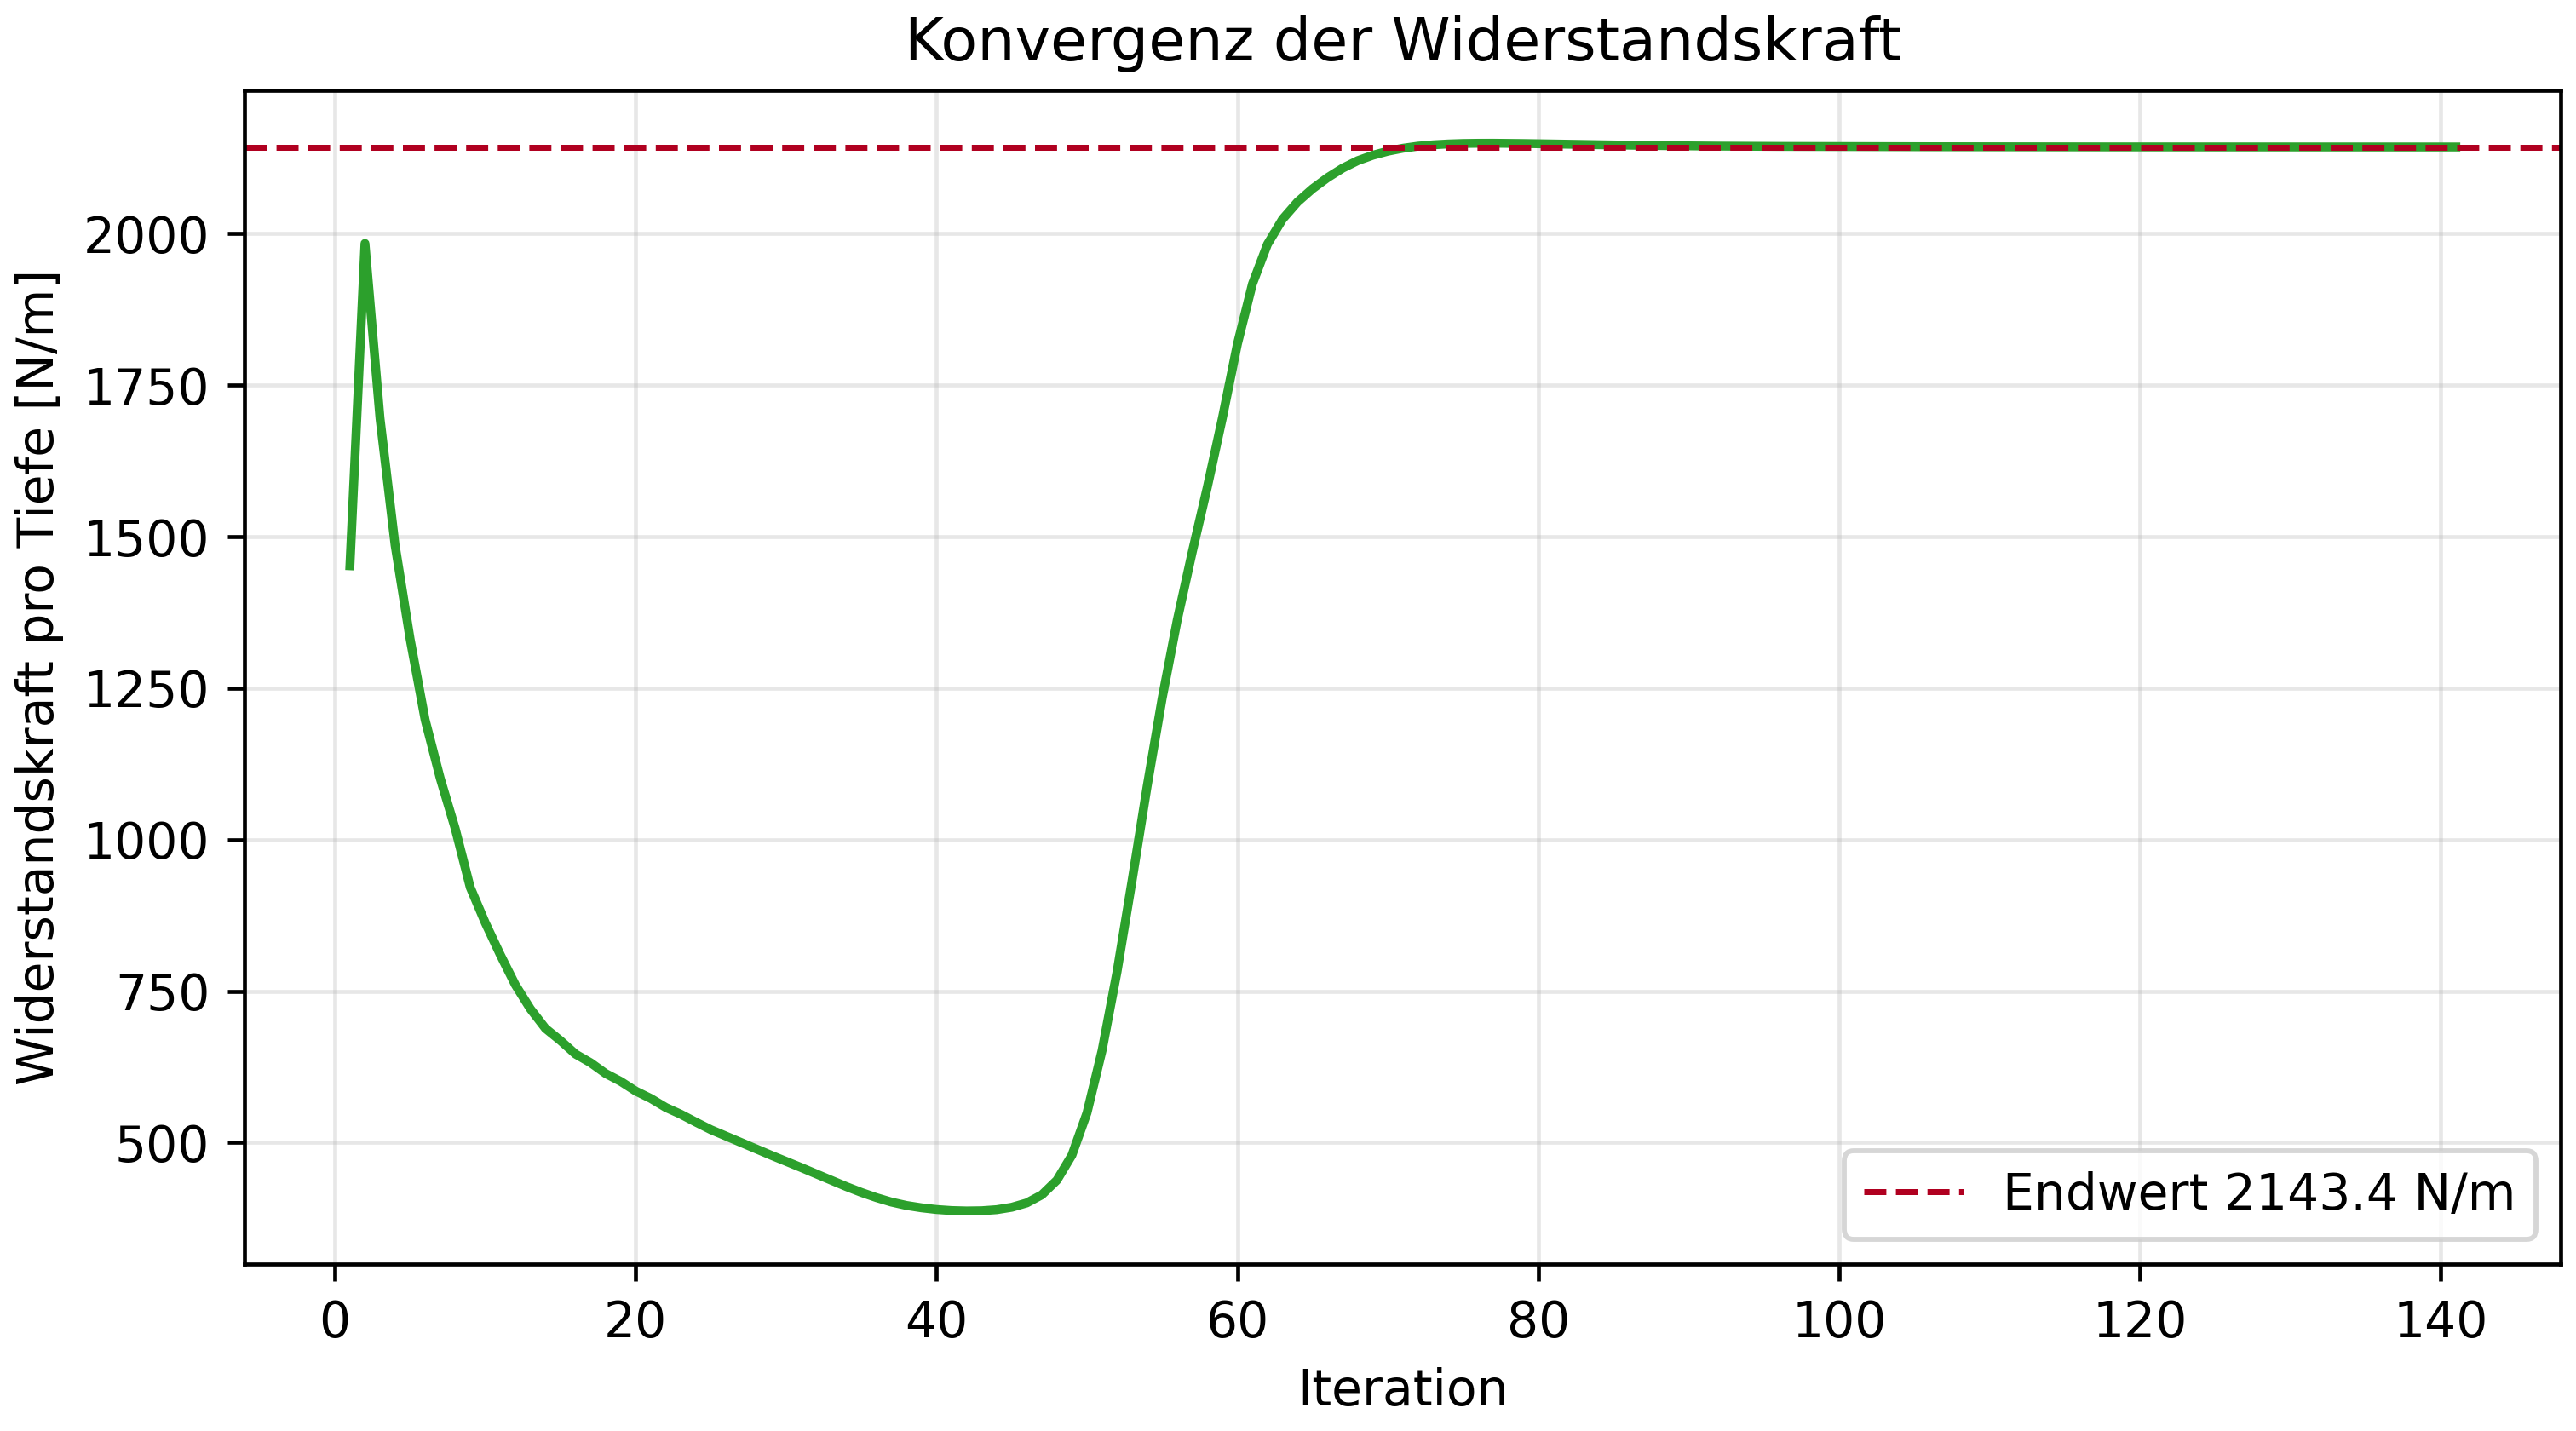
\includegraphics[width=\linewidth]{Aufgabe1/figures/drag_convergence.png}\caption{Widerstandskonvergenz}\end{subfigure}
\end{figure}

Die Integration der exportierten Wanddruckwerte ergibt \(6428.9\,\mathrm{N}\), der Fluent-Kraftreport \(6430.05\,\mathrm{N}\); die Abweichung beträgt nur \(0.02\,\%\). Der Kraftmonitor ist anfangs nicht monoton, weil sich Nachlauf und Druckfeld erst ausbilden. Maßgebend ist die stabile Endphase; in den letzten 20 Iterationen schwankt \(c_D\) nur noch um etwa \(0.0036\,\%\).

\subsection*{1.1 e)--f) Widerstandskraft und Widerstandsbeiwert}
Fluent liefert für die zweidimensionale Rechnung
\[
F'_D=2143.3515\,\mathrm{N/m}.
\]
Mit der Schildbreite \(3\,\mathrm{m}\) ergibt sich
\[
F_D=6430.05\,\mathrm{N},\qquad
c_D=\frac{F_D}{qA}=\frac{6430.05}{571.86\cdot6.0}=1.874.
\]
Zum Literaturvergleich nennt das \textit{Lexikon der Physik} (Spektrum, Stichwort ``Plattenumstroemung'', \url{https://www.spektrum.de/lexikon/physik/plattenumstroemung/11390}) fuer eine quer angestroemte Platte mit Abloesung \(c_w\approx 1{,}1\) bis \(1{,}3\). \(c_D=1{,}874\) liegt darueber, bleibt aber in der Groessenordnung stumpfer Platten mit Kantenabloesung; plausibel wegen endlicher Platte, scharfer Kanten und vollem Nachlauf. Aus \(\bar p_\mathrm{vorne}\approx 636\,\mathrm{Pa}\), \(\bar p_\mathrm{hinten}\approx -436\,\mathrm{Pa}\) folgt ebenfalls \(c_D\approx 1{,}87\).

\begin{table}[H]\centering\small
\begin{tabular}{lrr}
\toprule
Anteil & Kraft [N] & Bewertung\\
\midrule
Druckwiderstand & \(6430.090\) & maßgebend\\
Reibungsanteil & \(-0.036\) & vernachlässigbar\\
Summe & \(6430.054\) & Last für Strukturmodell\\
\bottomrule
\end{tabular}
\end{table}

\section{Aufgabe 1.2: Strukturmechanische Berechnung}

\subsection*{1.2 a) Aluminiumtafel, Singularitäten und Lagerkonzept}
Die CFD-Kraft wird als gleichmäßig verteilte Flächenlast auf die Tafel übertragen:
\[
p=\frac{6430.05}{3000\cdot2000}=0.001071676\,\mathrm{N/mm^2}.
\]
Die Tafel wurde mit SHELL181, \(E=70000\,\mathrm{N/mm^2}\), \(\nu=0.3\) und \(t=3\,\mathrm{mm}\) modelliert. SHELL181 ist trotz ebenem Spannungszustand sinnvoll, weil die Windlast Plattenbiegung erzeugt; die Mittelebene bleibt bei \(t=3\,\mathrm{mm}\) dennoch maßgebend. Die zulässige Spannung beträgt
\[
\sigma_\mathrm{zul}=\frac{190}{1.8}=105.56\,\mathrm{MPa}.
\]

Punktlager erzeugen lokal sehr hohe Spannungen direkt am idealisierten Festhalteknoten. Der Singularitätsnachweis erfolgt deshalb über eine Netzstudie am gleichen Punktlager: Lagerposition und Verfeinerungszone bleiben geometrisch gleich, nur die lokale Netzgröße wird von \(10\,\mathrm{mm}\) auf \(2\,\mathrm{mm}\) und \(1\,\mathrm{mm}\) reduziert. Ausgewertet werden \(\sigma_{v,\max}\) und die nodale Tributärfläche mit \(\sigma_v>\sigma_\mathrm{zul}\).

\begin{table}[H]\centering\small
\begin{tabular}{rrrrrr}
\toprule
lokale Netzgroesse [mm] & Knoten & Elemente & $\sigma_{v,\max}$ [MPa] & $A(\sigma_v>\sigma_\mathrm{zul})$ [mm$^2$] & Status\\
\midrule
10 & 7985 & 15768 & 729.41 & 2612031.4 & ausgewertet\\
2 & 29525 & 58848 & 967.60 & 2613774.7 & ausgewertet\\
1 & 56450 & 112698 & 1070.70 & 2609452.9 & ausgewertet\\
\bottomrule
\end{tabular}

\caption{Netzstudie für die Punktlager. Die Zeilen werden nach dem MAPDL-Solverlauf automatisch mit Spannungsmaximum und überlasteter Fläche gefüllt.}
\end{table}

Der maßgebende Singularitätsindikator ist das Spannungsmaximum am Punktlager: Bei unveränderter Lagergeometrie steigt \(\sigma_{v,\max}\) von \(729.41\,\mathrm{MPa}\) über \(967.60\,\mathrm{MPa}\) auf \(1070.70\,\mathrm{MPa}\), wenn die lokale Netzgröße von \(10\,\mathrm{mm}\) auf \(2\,\mathrm{mm}\) und \(1\,\mathrm{mm}\) reduziert wird. Die überlastete Gesamtfläche ist dagegen kein isolierter Singularitätsindikator, weil sie auch die globale Biegebeanspruchung der Tafel enthält.

\begin{figure}[H]
\centering
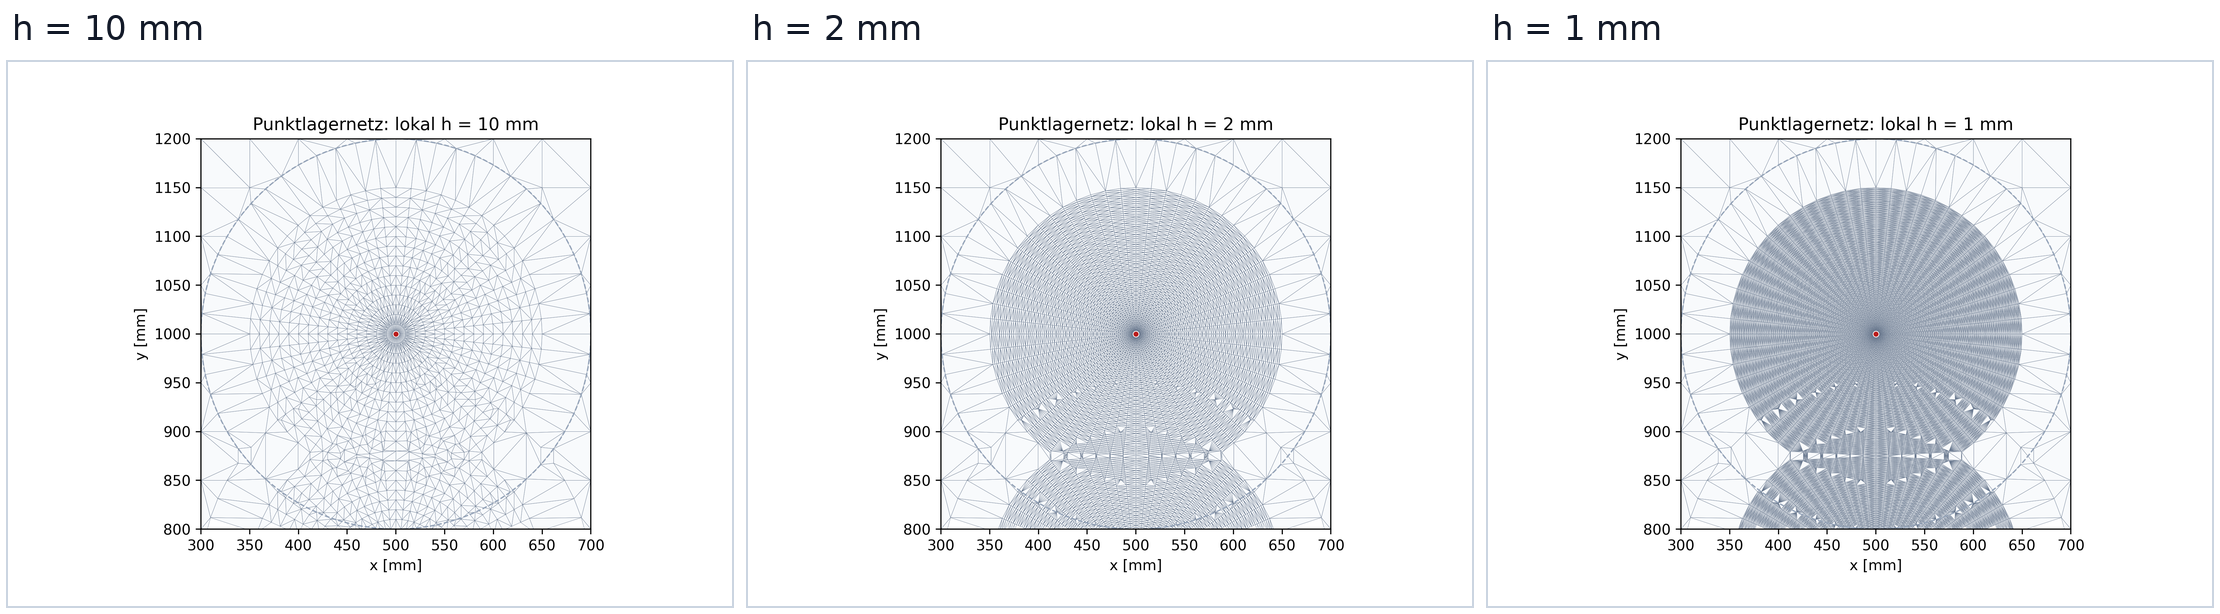
\includegraphics[width=\linewidth]{Aufgabe1/figures/plate_singularity_mesh_panel.png}
\caption{Drei Netzvarianten für den Singularitätsnachweis am Punktlager: Die lokale Verfeinerungszone bleibt in allen Varianten gleich groß; nur die Netzgröße wird verändert.}
\end{figure}

\IfFileExists{../Aufgabe1/figures/plate_singularity_stress_panel.png}{
\begin{figure}[H]
\centering
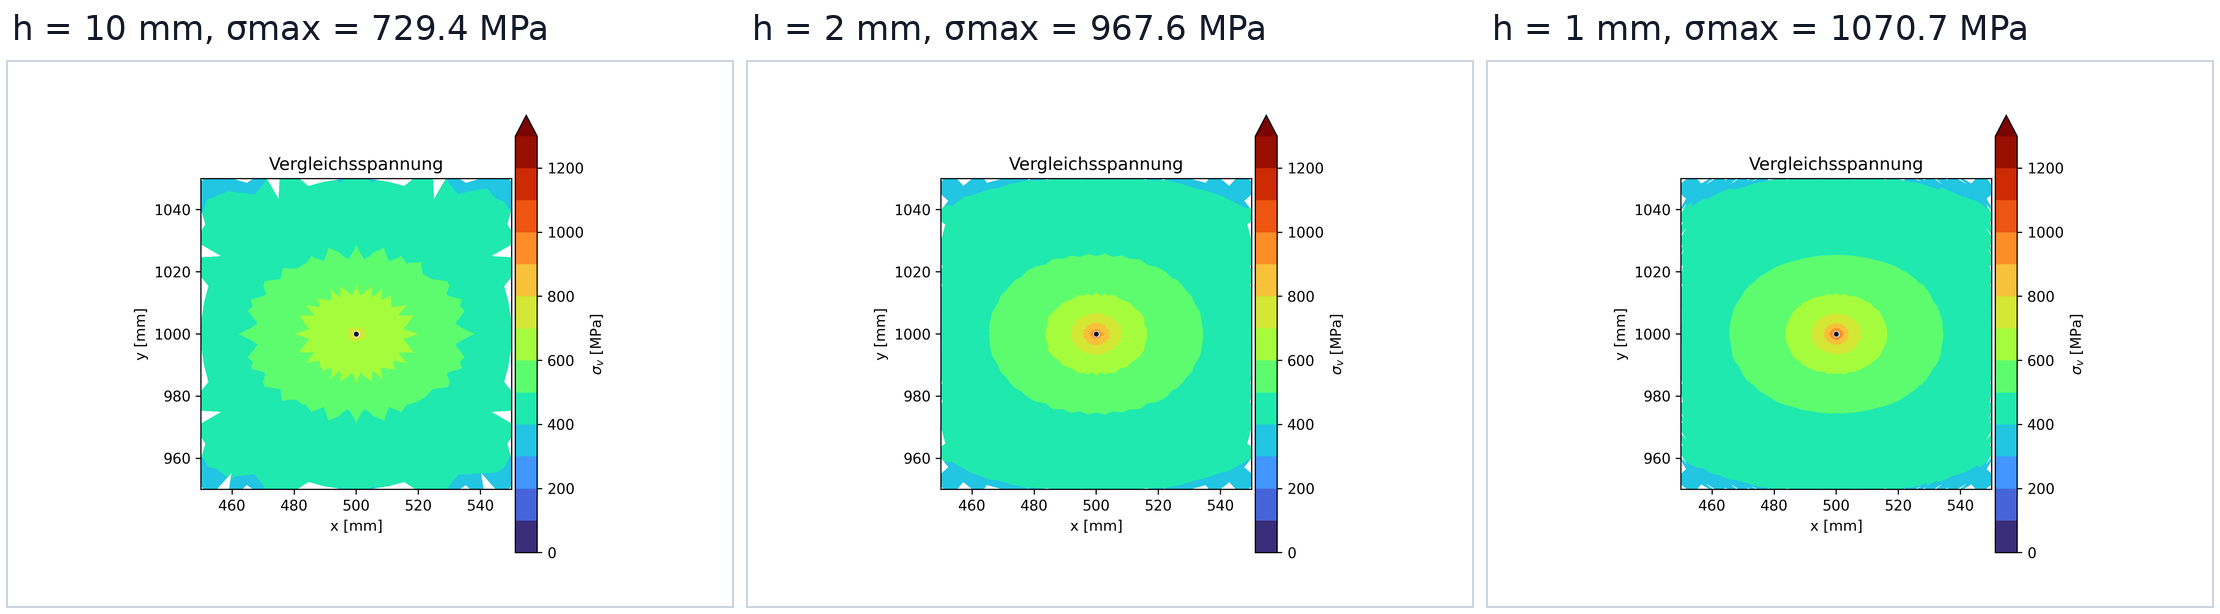
\includegraphics[width=\linewidth]{Aufgabe1/figures/plate_singularity_stress_panel.png}
\caption{Vergleichsspannung der drei Punktlager-Netzvarianten. Die Spannungsspitze liegt am idealisierten Festhalteknoten und ist deshalb randbedingungsdominiert.}
\end{figure}
}{
\begin{center}\small
\textit{Die Spannungsbilder der drei Punktlager-Netzvarianten werden nach dem MAPDL-Export automatisch unter der Netzabbildung eingefügt.}
\end{center}
}

Die Studie wird mit \texttt{run\_plate\_singularity\_study.py} erzeugt; \texttt{parse\_plate\_structural\_results.py} kombiniert die MAPDL-Spannungen mit den Elementflächen. Damit hängt die Singularitätsaussage nicht nur von der Farbskala eines Konturplots ab.

Für die konstruktive Bewertung wurde die Tafel zusätzlich mit vertikalen Linienstützen untersucht:
\begin{itemize}
\item \textbf{Punktlager:} mathematisch harte Lagerung an einzelnen Knoten; geeignet zum Erkennen der Singularität, aber nicht als realer Spannungsnachweis der Tafel.
\item \textbf{Vertikale Linienstützen bzw. Stäbe/Profile:} idealisierte Rückseitenprofile bzw. durchgehende Tragleisten; diese entsprechen eher der Tragstruktur realer Autobahnschilder.
\end{itemize}

Die hohen Spannungen bei Punktlagern sind randbedingungsdominiert und kein robuster Nachweis für die Gesamttafel. Entscheidend für ein mögliches konstruktives Lagerkonzept sind Spannungsbild, Verformung und Lastreaktionen der Linienstützen bzw. Stäbe.

\begin{table}[H]\centering\small
\begin{tabular}{lrrrr}
\toprule
Modell & lokale Netzgröße & Lagerknoten/Lager & \(\sigma_{v,\max}\) [MPa] & \(u_{z,\max}\) [mm]\\
\midrule
Linienstützen & \(50\,\mathrm{mm}\) Raster & Linie & 63.77 & 40.30\\
\bottomrule
\end{tabular}
\end{table}

Als realistischere Konstruktion wurden drei vertikale \(50\,\mathrm{mm}\) breite Linienstützen an den Fachwerkpositionen \(x=500,1500,2500\,\mathrm{mm}\) modelliert. Sie bilden die Aussteifung realer Rückseitenprofile vereinfacht ab.

\begin{figure}[H]
\centering
\begin{subfigure}{0.32\linewidth}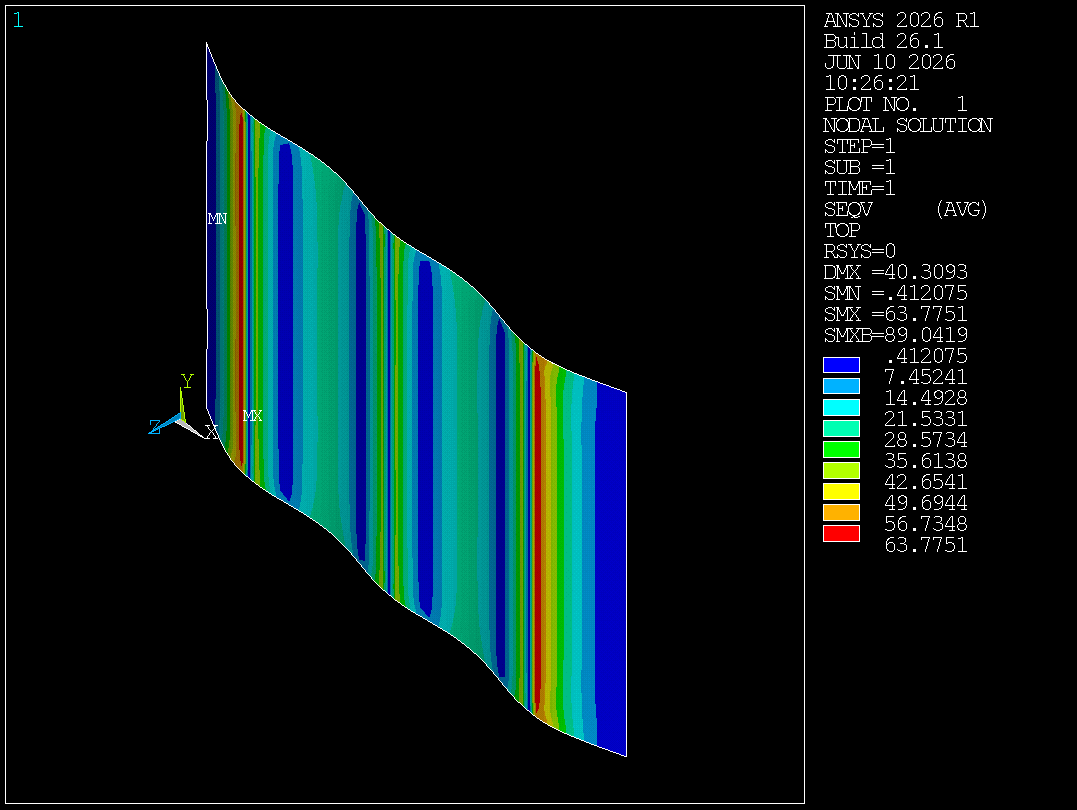
\includegraphics[width=\linewidth]{Aufgabe1/data/plate_line_support_full_height/plate_spannung_eqv_ansys.png}\caption{Linienstützen: Spannung}\end{subfigure}
\begin{subfigure}{0.32\linewidth}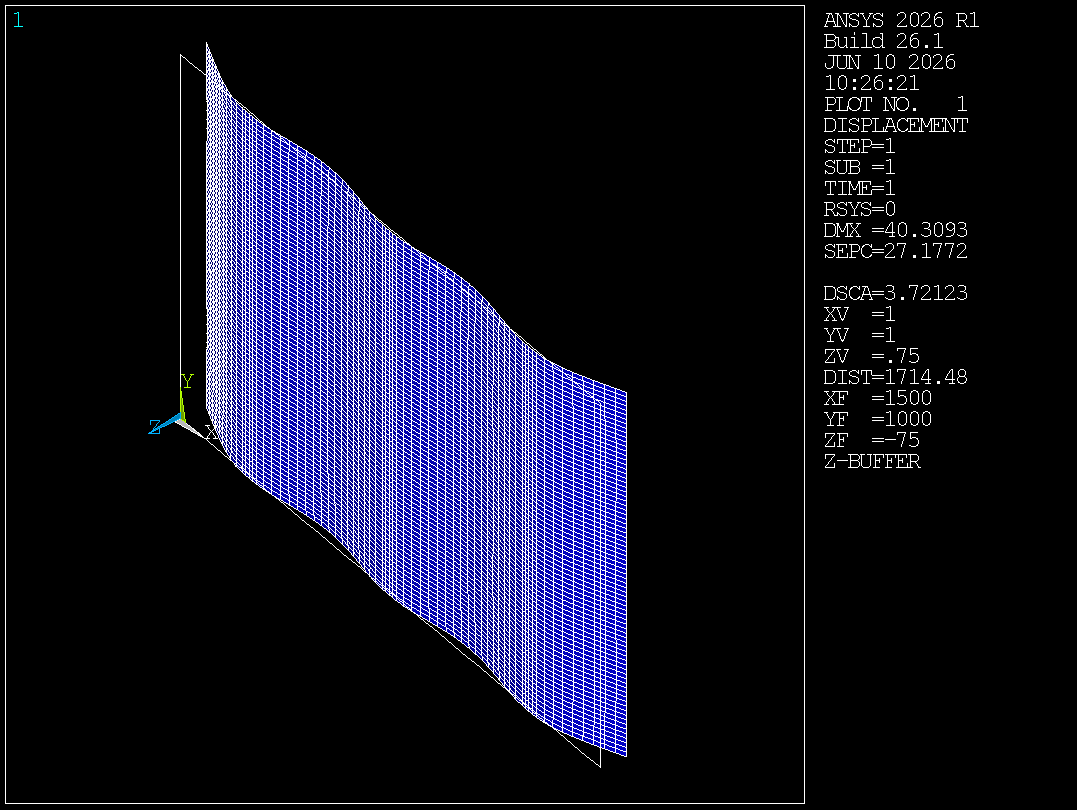
\includegraphics[width=\linewidth]{Aufgabe1/data/plate_line_support_full_height/plate_verformung_ansys.png}\caption{Linienstützen: Verformung}\end{subfigure}
\begin{subfigure}{0.32\linewidth}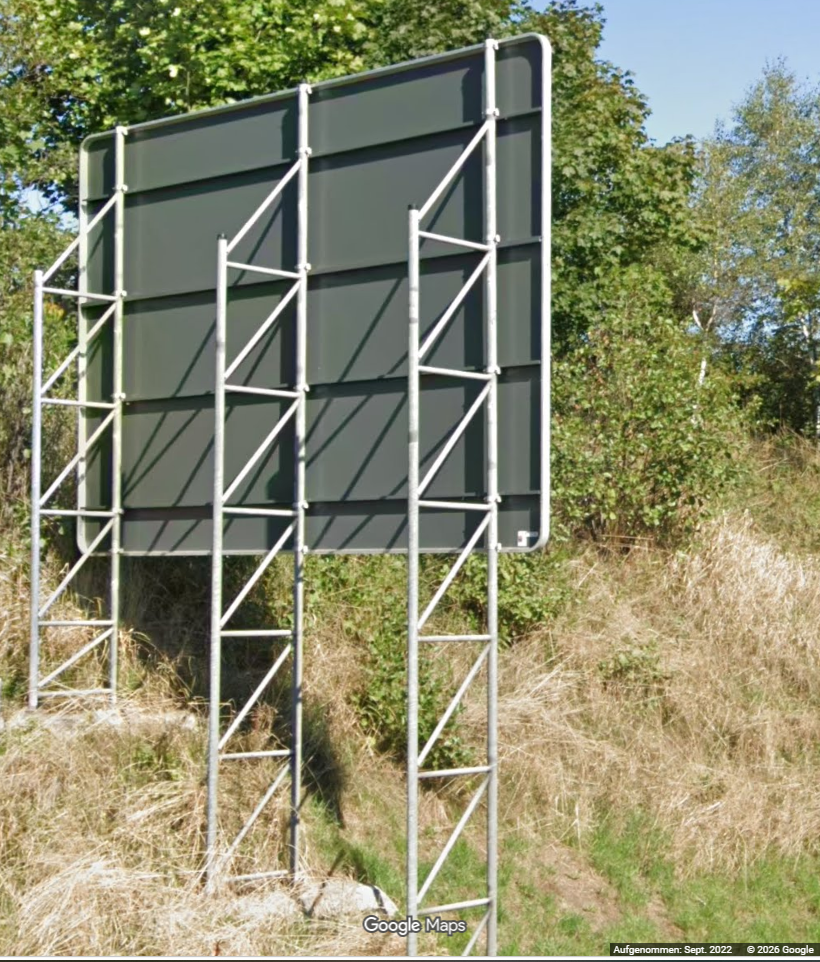
\includegraphics[width=\linewidth]{Aufgabe1/figures/A9_Schild_von_hinten_genommen.PNG}\caption{Rückseite (Google Street View, Copyright Google)}\end{subfigure}
\caption{Konstruktiv maßgebendes Linienlager und reale Rückseitenprofile. Die Punktlager werden oben nur für den Singularitätsnachweis verwendet.}
\end{figure}

Für dieses Lagerkonzept gilt:
\[
\sigma_{v,\max}=63.77\,\mathrm{MPa},\quad
u_{z,\max}=40.30\,\mathrm{mm},\quad
\sigma_{v,\max}/\sigma_\mathrm{zul}=0.604.
\]
Die Tafel ist ausreichend dimensioniert, weil \(\sigma_{v,\max}<\sigma_\mathrm{zul}\) gilt. Die Linienlagerreaktionen \(2144.94\,\mathrm{N}\), \(2140.18\,\mathrm{N}\), \(2144.94\,\mathrm{N}\) summieren sich zu \(6430.05\,\mathrm{N}\) und stimmen mit der CFD-Windkraft überein.

Für die Lastweitergabe auf das Fachwerk wurde zusätzlich das Aufgabenmodell mit gelenkiger Anbindung an die obersten zwei Knoten je Träger gerechnet:

\begin{table}[H]\centering\small
\begin{tabular}{lrrr}
\toprule
Träger & \(F_\mathrm{oben}\) [N] & \(F_\mathrm{unten}\) [N] & Summe [N]\\
\midrule
H1 & 1604.90 & 540.84 & 2145.74\\
H2 & 1606.75 & 533.15 & 2139.90\\
H3 & 1604.90 & 540.84 & 2145.74\\
\bottomrule
\end{tabular}
\end{table}
Maßgebend für die Fachwerkdimensionierung ist Träger H3 (höchste Trägerreaktion, gemeinsam mit H1). Für die weitere Berechnung werden dessen Gelenkkräfte \(P_\mathrm{oben}=1604.90\,\mathrm{N}\) und \(P_\mathrm{unten}=540.84\,\mathrm{N}\) verwendet.

\subsection*{1.2 b) Normalkräfte aus ANSYS}
Das Fachwerk bleibt ein Gelenkstabwerk, belastet über die Gelenkkräfte \(P_\mathrm{oben}=1604.90\,\mathrm{N}\), \(P_\mathrm{unten}=540.84\,\mathrm{N}\). Die maximalen ANSYS-Normalkräfte sind:
\[
N_\mathrm{vert}=8044.10\,\mathrm{N},\quad
N_\mathrm{horiz}=2145.70\,\mathrm{N},\quad
N_\mathrm{diag}=2454.60\,\mathrm{N}.
\]

\subsection*{1.2 c) Ritter-Schnitt}
Mit Momentengleichgewicht um \(L0\):
\[
R_{R0,y}=-\frac{1604.90\cdot7h+540.84\cdot6h}{b}=-8044.10\,\mathrm{N}.
\]
Daraus folgen \(R_{L0,y}=8044.10\,\mathrm{N}\) und \(R_{L0,x}=2145.74\,\mathrm{N}\). Für die Diagonale gilt
\[
l_D=\sqrt{0.45^2+0.25^2}=0.5148\,\mathrm{m},\quad
\cos\alpha=0.8742,\quad
N_D=\frac{2145.74}{0.8742}=2454.52\,\mathrm{N}.
\]
Die Handrechnung bestätigt damit die Größenordnung der ANSYS-Stabkräfte.

\subsection*{1.2 d) Dimensionierung der Fachwerkstäbe}
Für Stahl wird \(\sigma_\mathrm{zul}=235/1.8=130.56\,\mathrm{MPa}\) angesetzt. Die Rohrquerschnitte wurden so gewählt, dass die vorhandenen Spannungen unterhalb der zulässigen Spannung bleiben.

\begin{table}[H]\centering\small
\begin{tabular}{lrrrrrr}
\toprule
Gruppe & \(N_{\max}\) [N] & \(A_\mathrm{erf}\) [mm\(^2\)] & Außen-Ø [mm] & Innen-Ø [mm] & Wand [mm] & \(\sigma\) [MPa]\\
\midrule
vertikal & 8044.10 & 61.61 & 16 & 13 & 1.5 & 117.73\\
horizontal & 2145.74 & 16.44 & 12 & 9 & 1.5 & 43.36\\
diagonal & 2454.52 & 18.80 & 12 & 9 & 1.5 & 49.60\\
\bottomrule
\end{tabular}
\end{table}

\subsection*{1.2 e)--h) Eigenes Python-FEM und Vergleich}
Für den Vergleich wurden zwei getrennte Rechnungen mit gleicher Geometrie, Querschnitten, Randbedingungen und Lasten durchgeführt: ANSYS mit LINK180-Stabelementen und Python mit eigener Assemblierung von \(KU=F\). Verglichen werden die elementweisen Größen \(N_i\) und \(\sigma_i\).

Das Python-Programm modelliert H3 mit sieben Feldern (\(7h\)) und linear elastischen Stäben (\(E=210000\,\mathrm{N/mm^2}\)). Jeder Knoten besitzt \((U_x,U_y)\); \(A=L0\), \(B=R7\).

\textbf{Indextafel (Auszug):}
\begin{table}[H]\centering\footnotesize
\begin{tabular}{llll}
\toprule
Element & Knoten & Globale DOFs & Art\\
\midrule
VL1 & L0--L1 & 0, 1, 4, 5 & vertikal\\
D1 & L0--R1 & 0, 1, 6, 7 & diagonal\\
H0 & L0--R0 & 0, 1, 2, 3 & horizontal\\
VR7 & R6--R7 & 26, 27, 28, 29 & vertikal\\
D7 & L6--R7 & 24, 25, 28, 29 & diagonal\\
\bottomrule
\end{tabular}
\end{table}

Für jedes Stabelement gilt die Elementsteifigkeitsmatrix
\[
K^{(e)}=\frac{EA}{l}\begin{bmatrix}
c^2&cs&-c^2&-cs\\ cs&s^2&-cs&-s^2\\ -c^2&-cs&c^2&cs\\ -cs&-s^2&cs&s^2
\end{bmatrix}.
\]
Die Assemblierung erfolgt über die Indextafel (\texttt{K[I[a],I[b]]+=Ke[a,b]}). Der Lastvektor \(F\) enthält die Windkräfte an den belasteten Knoten \(R6\) und \(R7\):
\(F_{R7,x}=-1604.90\,\mathrm{N}\), \(F_{R6,x}=-540.84\,\mathrm{N}\); alle übrigen Komponenten sind null. Die Randbedingungen sind \(U_{L0,x}=U_{L0,y}=0\) und \(U_{R0,y}=0\).

Das Lösen von \(KU=F\) liefert die Lagerreaktionen in \(A\) und die Verschiebungen in \(B\):
\[
R_{A,x}=R_{L0,x}=2145.74\,\mathrm{N},\quad
R_{A,y}=R_{L0,y}=8044.10\,\mathrm{N},\quad
R_{R0,y}=-8044.10\,\mathrm{N},
\]
\[
u_{B,x}=u_{R7,x}=-3.996\,\mathrm{mm},\quad
u_{B,y}=u_{R7,y}=0.545\,\mathrm{mm}.
\]

\begin{table}[H]\centering\small
\begin{tabular}{lr}
\toprule
Vergleichsgröße Python gegen ANSYS & Abweichung\\
\midrule
maximale Kraftabweichung & \(0.042\,\mathrm{N}\)\\
maximale Spannungsabweichung & \(0.0045\,\mathrm{MPa}\)\\
\bottomrule
\end{tabular}
\end{table}

Ein Auszug aus dem elementweisen Vergleich zeigt, dass Vorzeichen und Beträge der Stabkräfte übereinstimmen:

\begin{table}[H]\centering\footnotesize
\begin{tabular}{llrrrrr}
\toprule
Element & Art & $N_\mathrm{Py}$ [N] & $N_\mathrm{ANSYS}$ [N] & $\Delta N$ [N] & $\sigma_\mathrm{Py}$ [MPa] & $\sigma_\mathrm{ANSYS}$ [MPa]\\
\midrule
VR1 & vertikal & 8044.07 & 8044.10 & 0.027 & 117.725 & 117.720\\
H1 & horizontal & 2145.74 & 2145.70 & -0.039 & 43.366 & 43.366\\
D1 & diagonal & -2454.64 & -2454.60 & 0.037 & -49.609 & -49.609\\
VL3 & vertikal & -4467.84 & -4467.80 & 0.042 & -65.387 & -65.387\\
\bottomrule
\end{tabular}

\caption{Elementweiser Auszug aus dem Vergleich zwischen eigener Python-FEM-Rechnung und ANSYS-MAPDL. \(\Delta N=N_\mathrm{ANSYS}-N_\mathrm{Py}\).}
\end{table}

Die sehr kleinen Differenzen entstehen nur durch Rundung der aus ANSYS gedruckten Tabellenwerte. Damit ist das eigene Programm für dieses lineare Stabwerksproblem verifiziert.

\begin{figure}[H]
\centering
\begin{subfigure}{0.48\linewidth}\centering
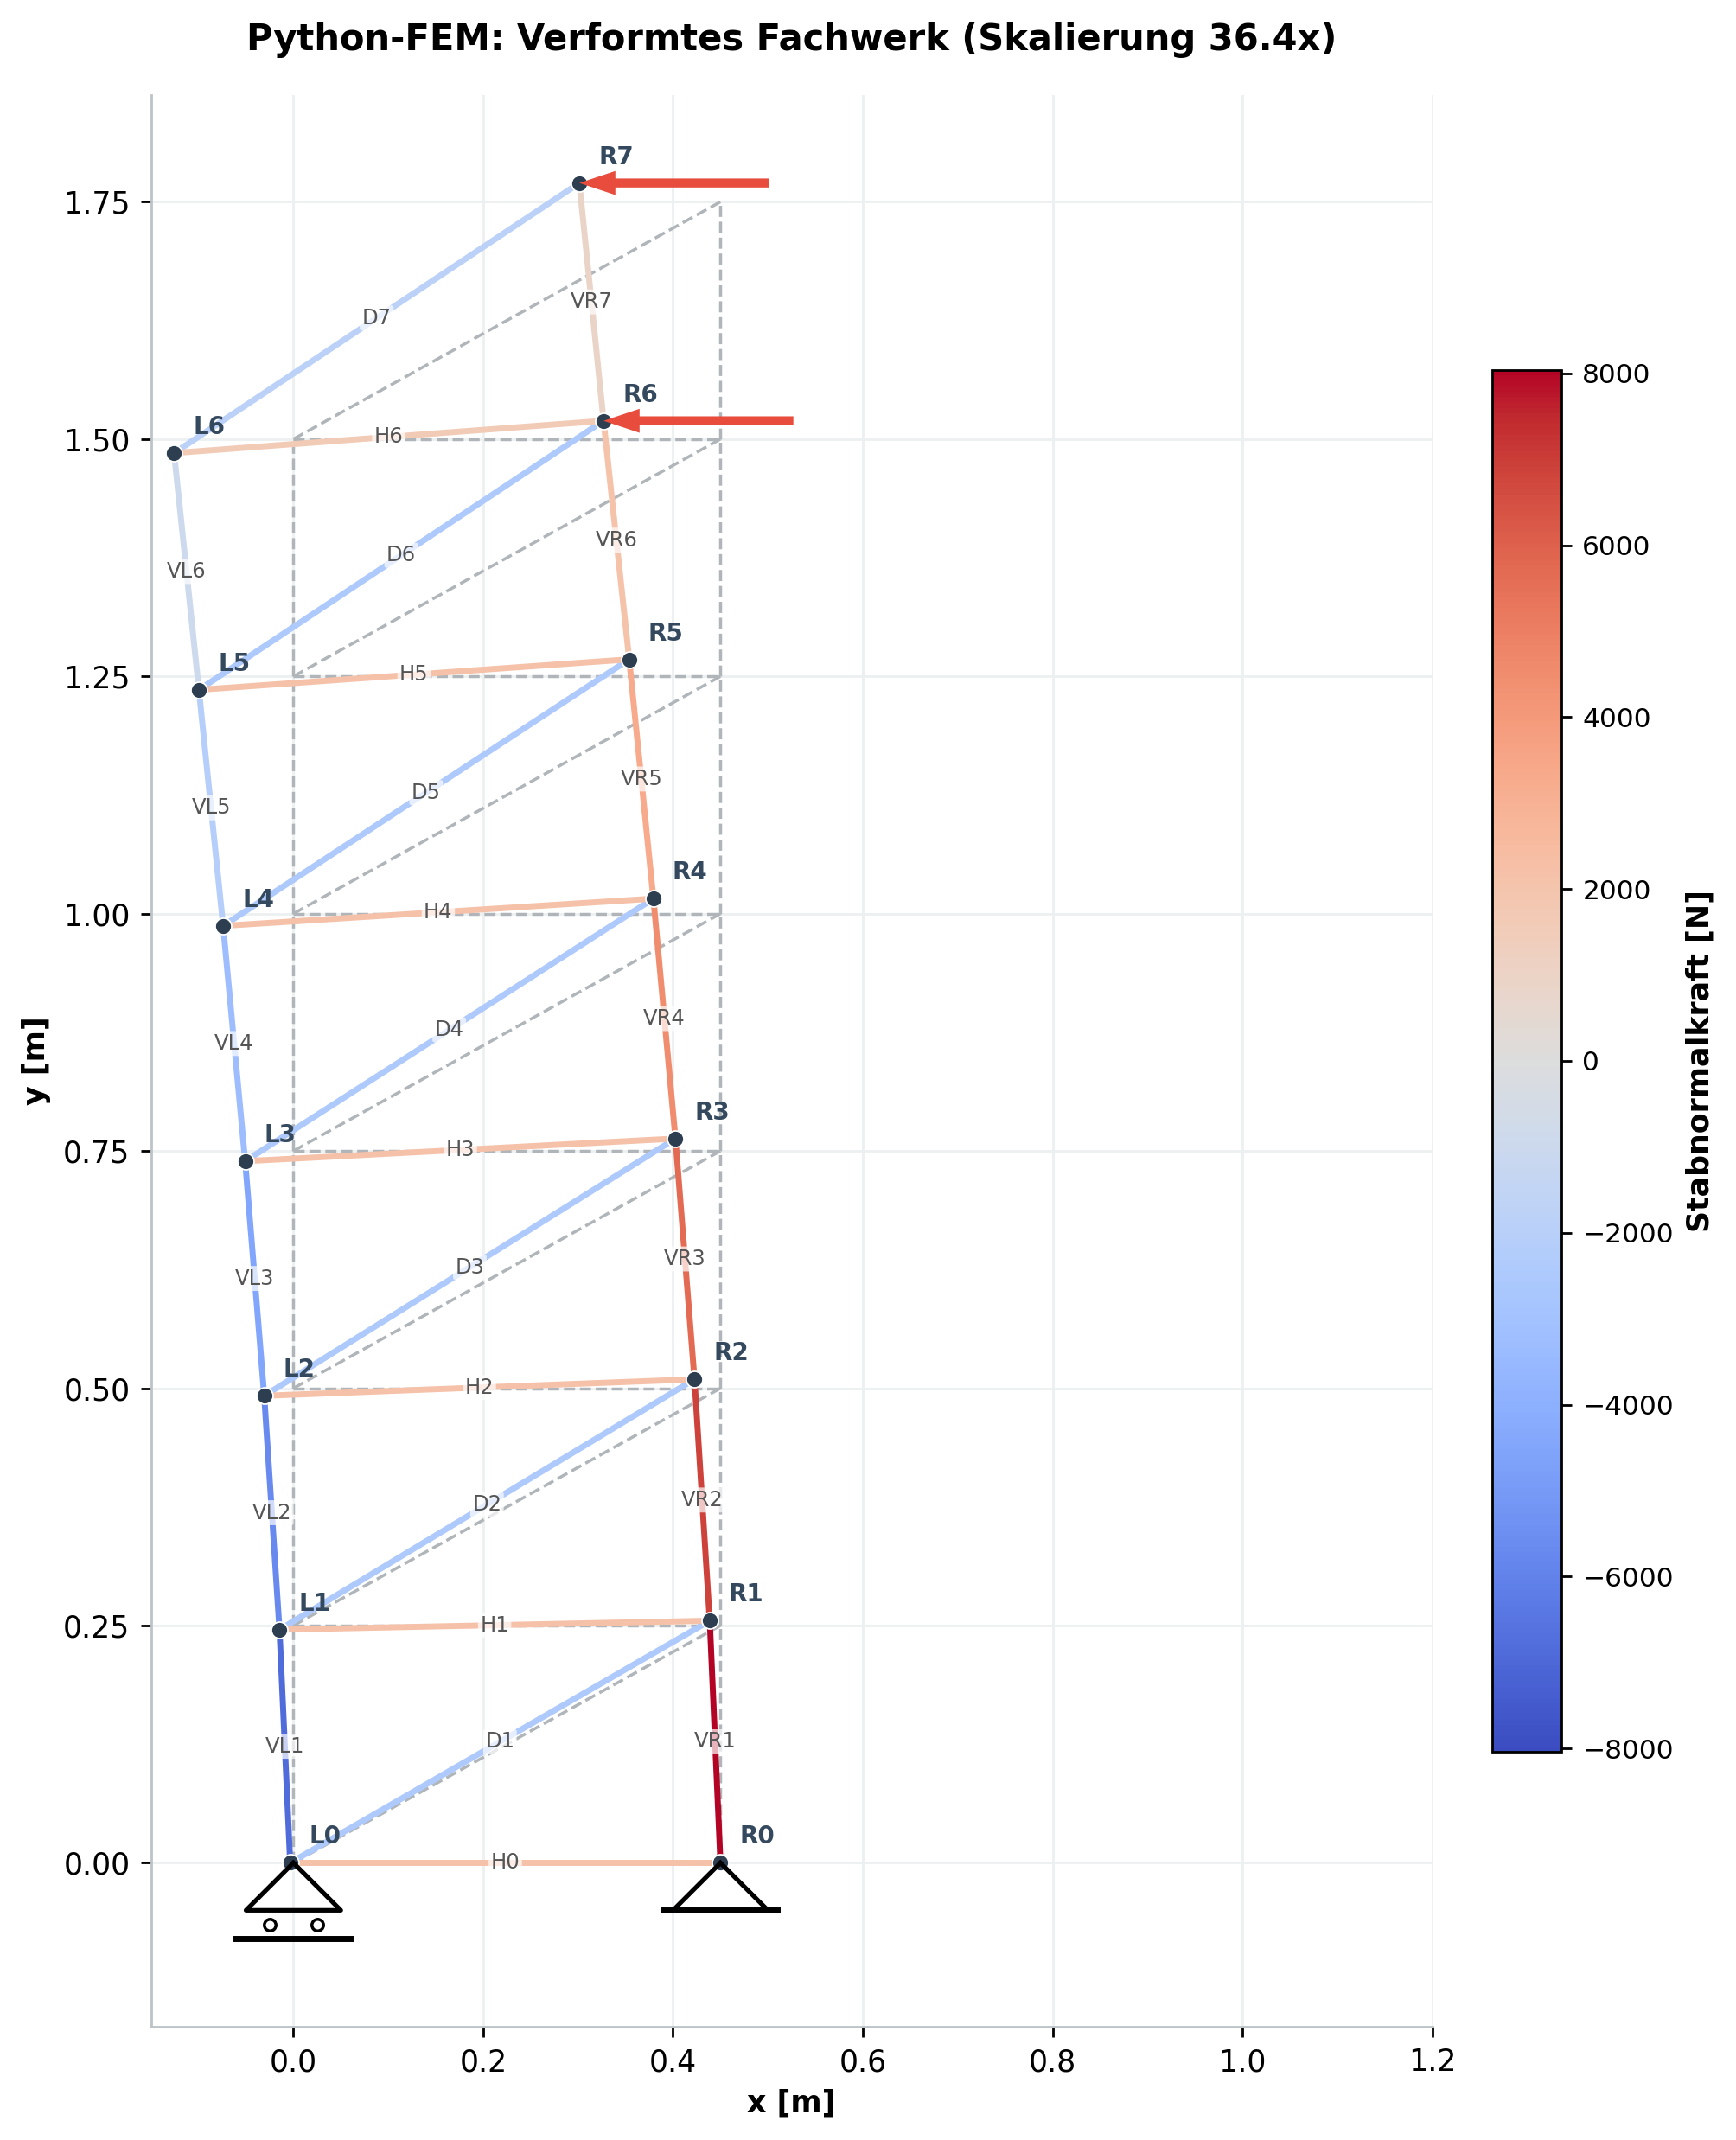
\includegraphics[height=0.25\textheight]{Aufgabe1/figures/truss_deformed.png}
\caption{Python-FEM}
\end{subfigure}
\begin{subfigure}{0.48\linewidth}\centering
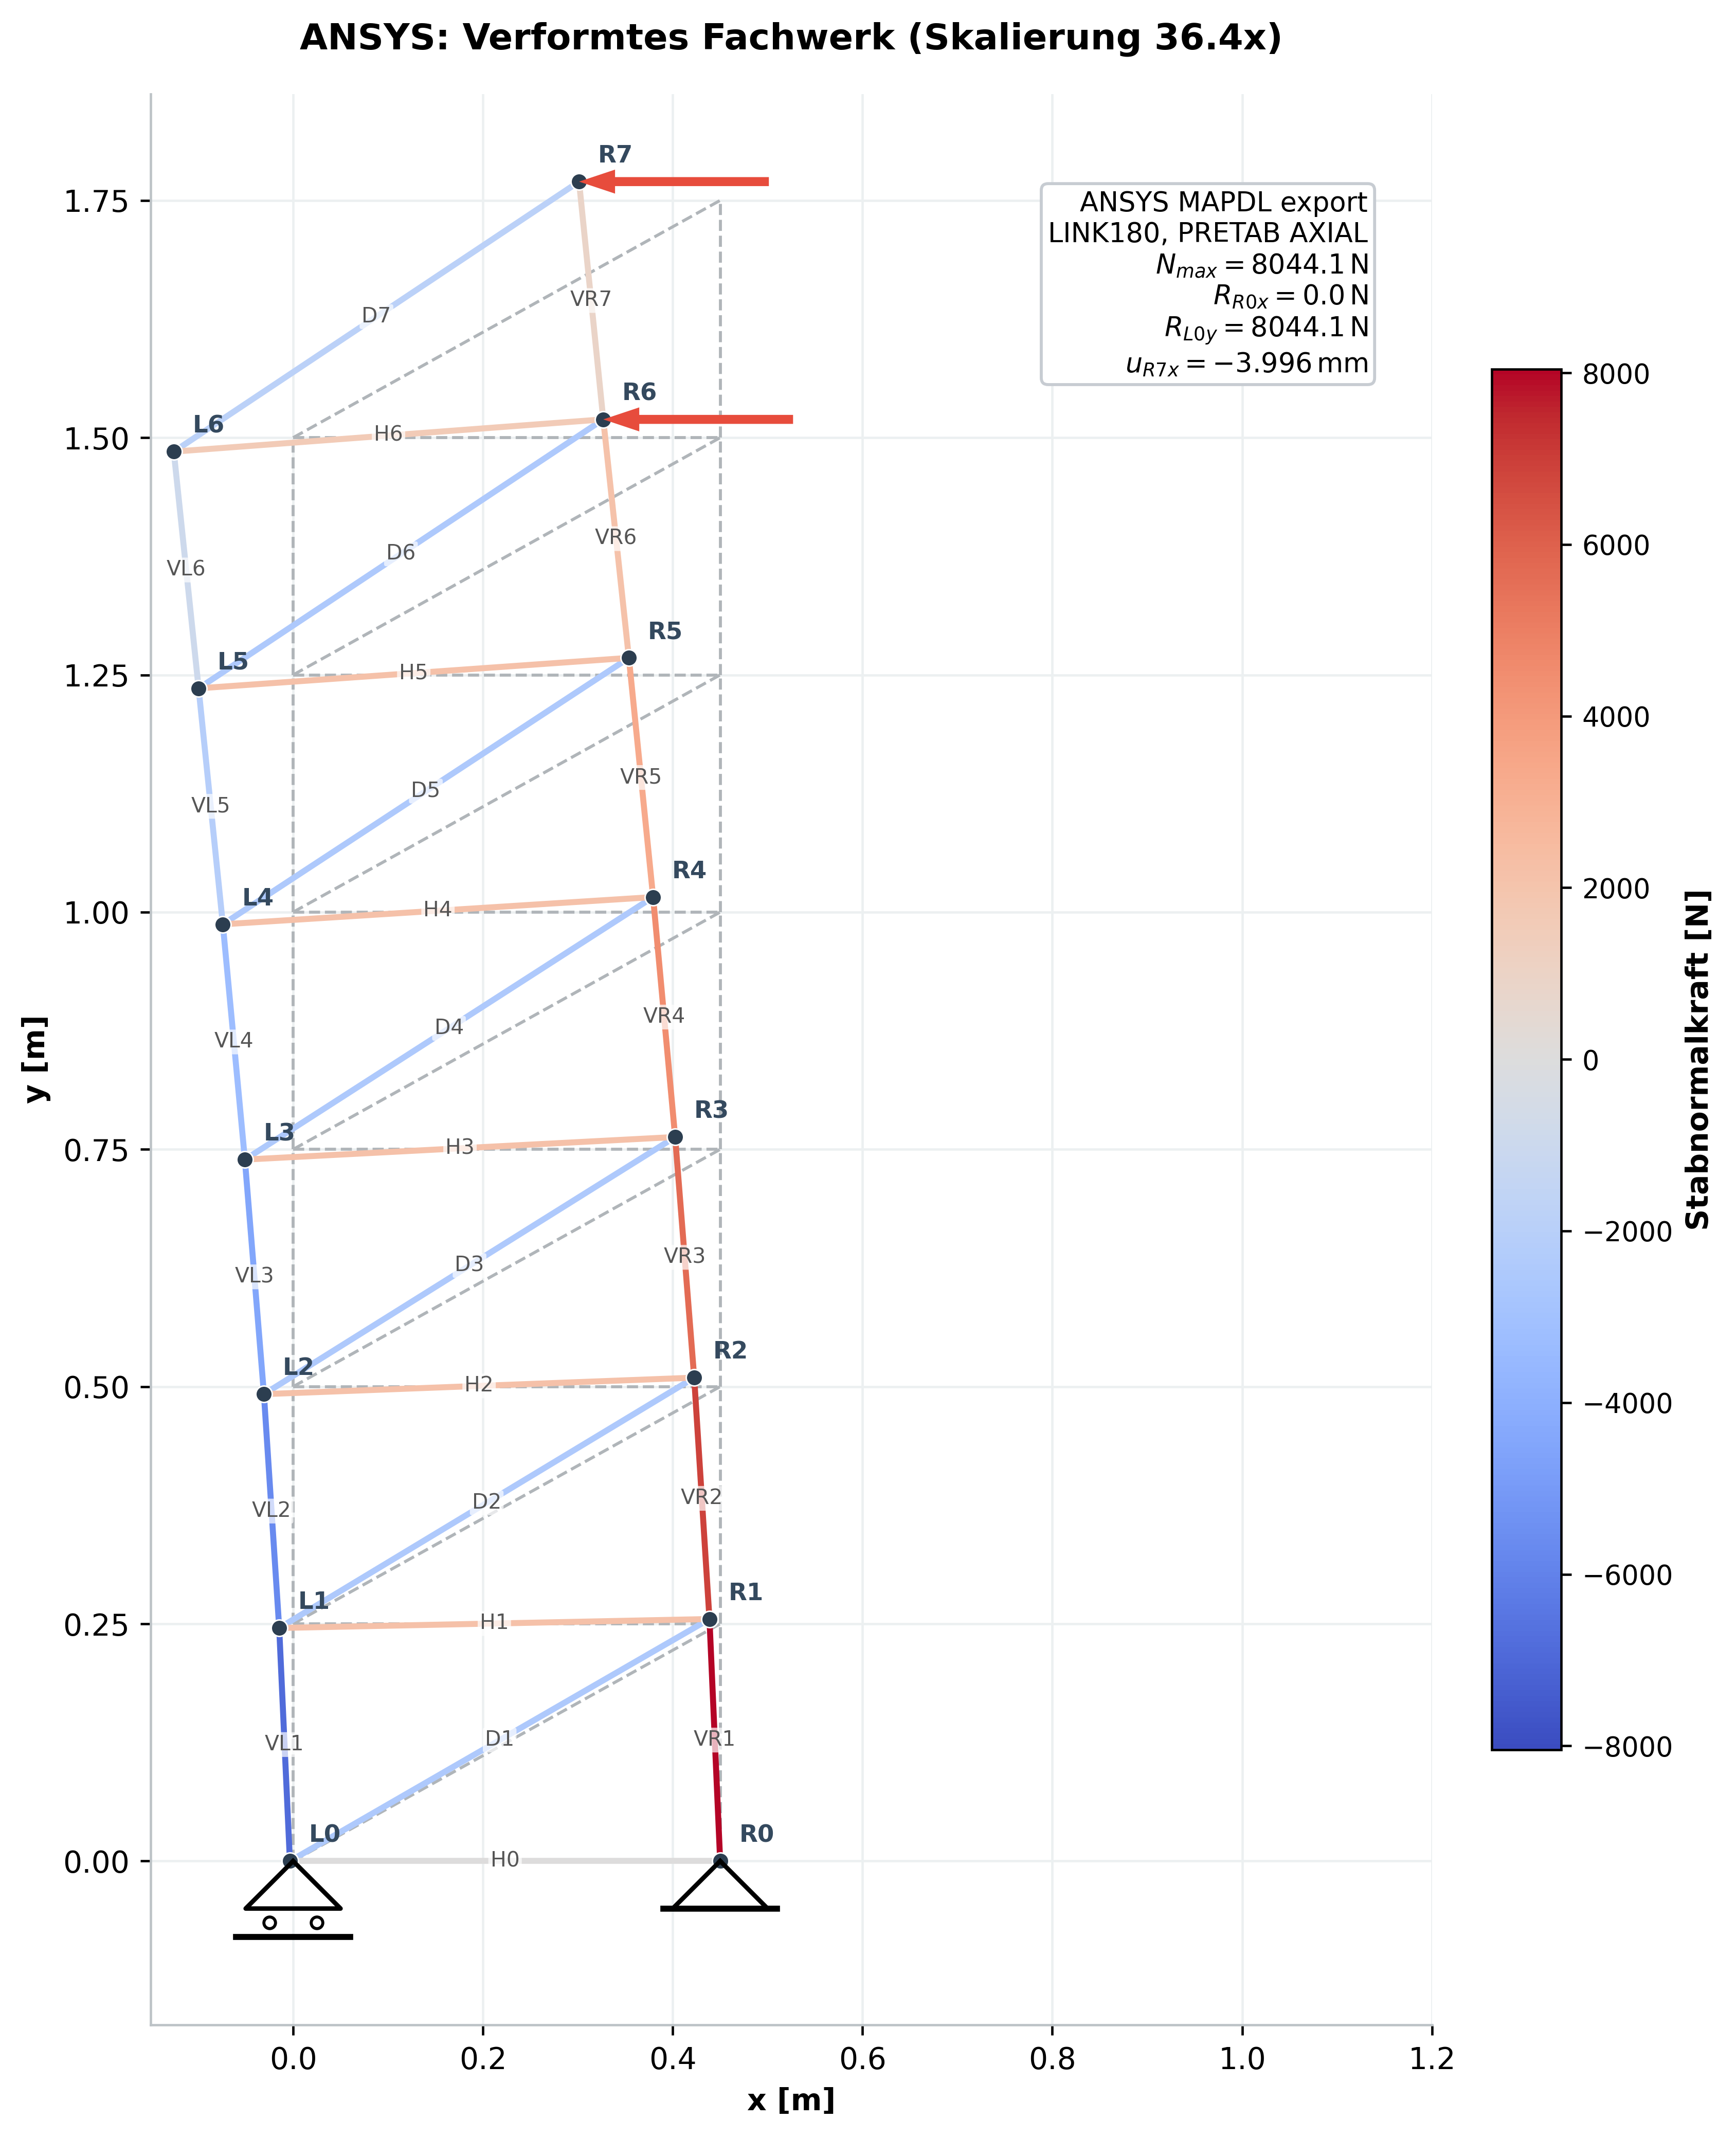
\includegraphics[height=0.25\textheight]{Aufgabe1/figures/truss_ansys_force_plot.png}
\caption{ANSYS-MAPDL-Export}
\end{subfigure}
\caption{Visueller Nachweis der Stabwerksrechnungen. Links die Python-Verformung, rechts die aus der ANSYS-Elementtabelle exportierten Normalkräfte mit Reaktionen. Rot bedeutet Zug, blau Druck.}
\end{figure}

\begin{figure}[H]
\centering
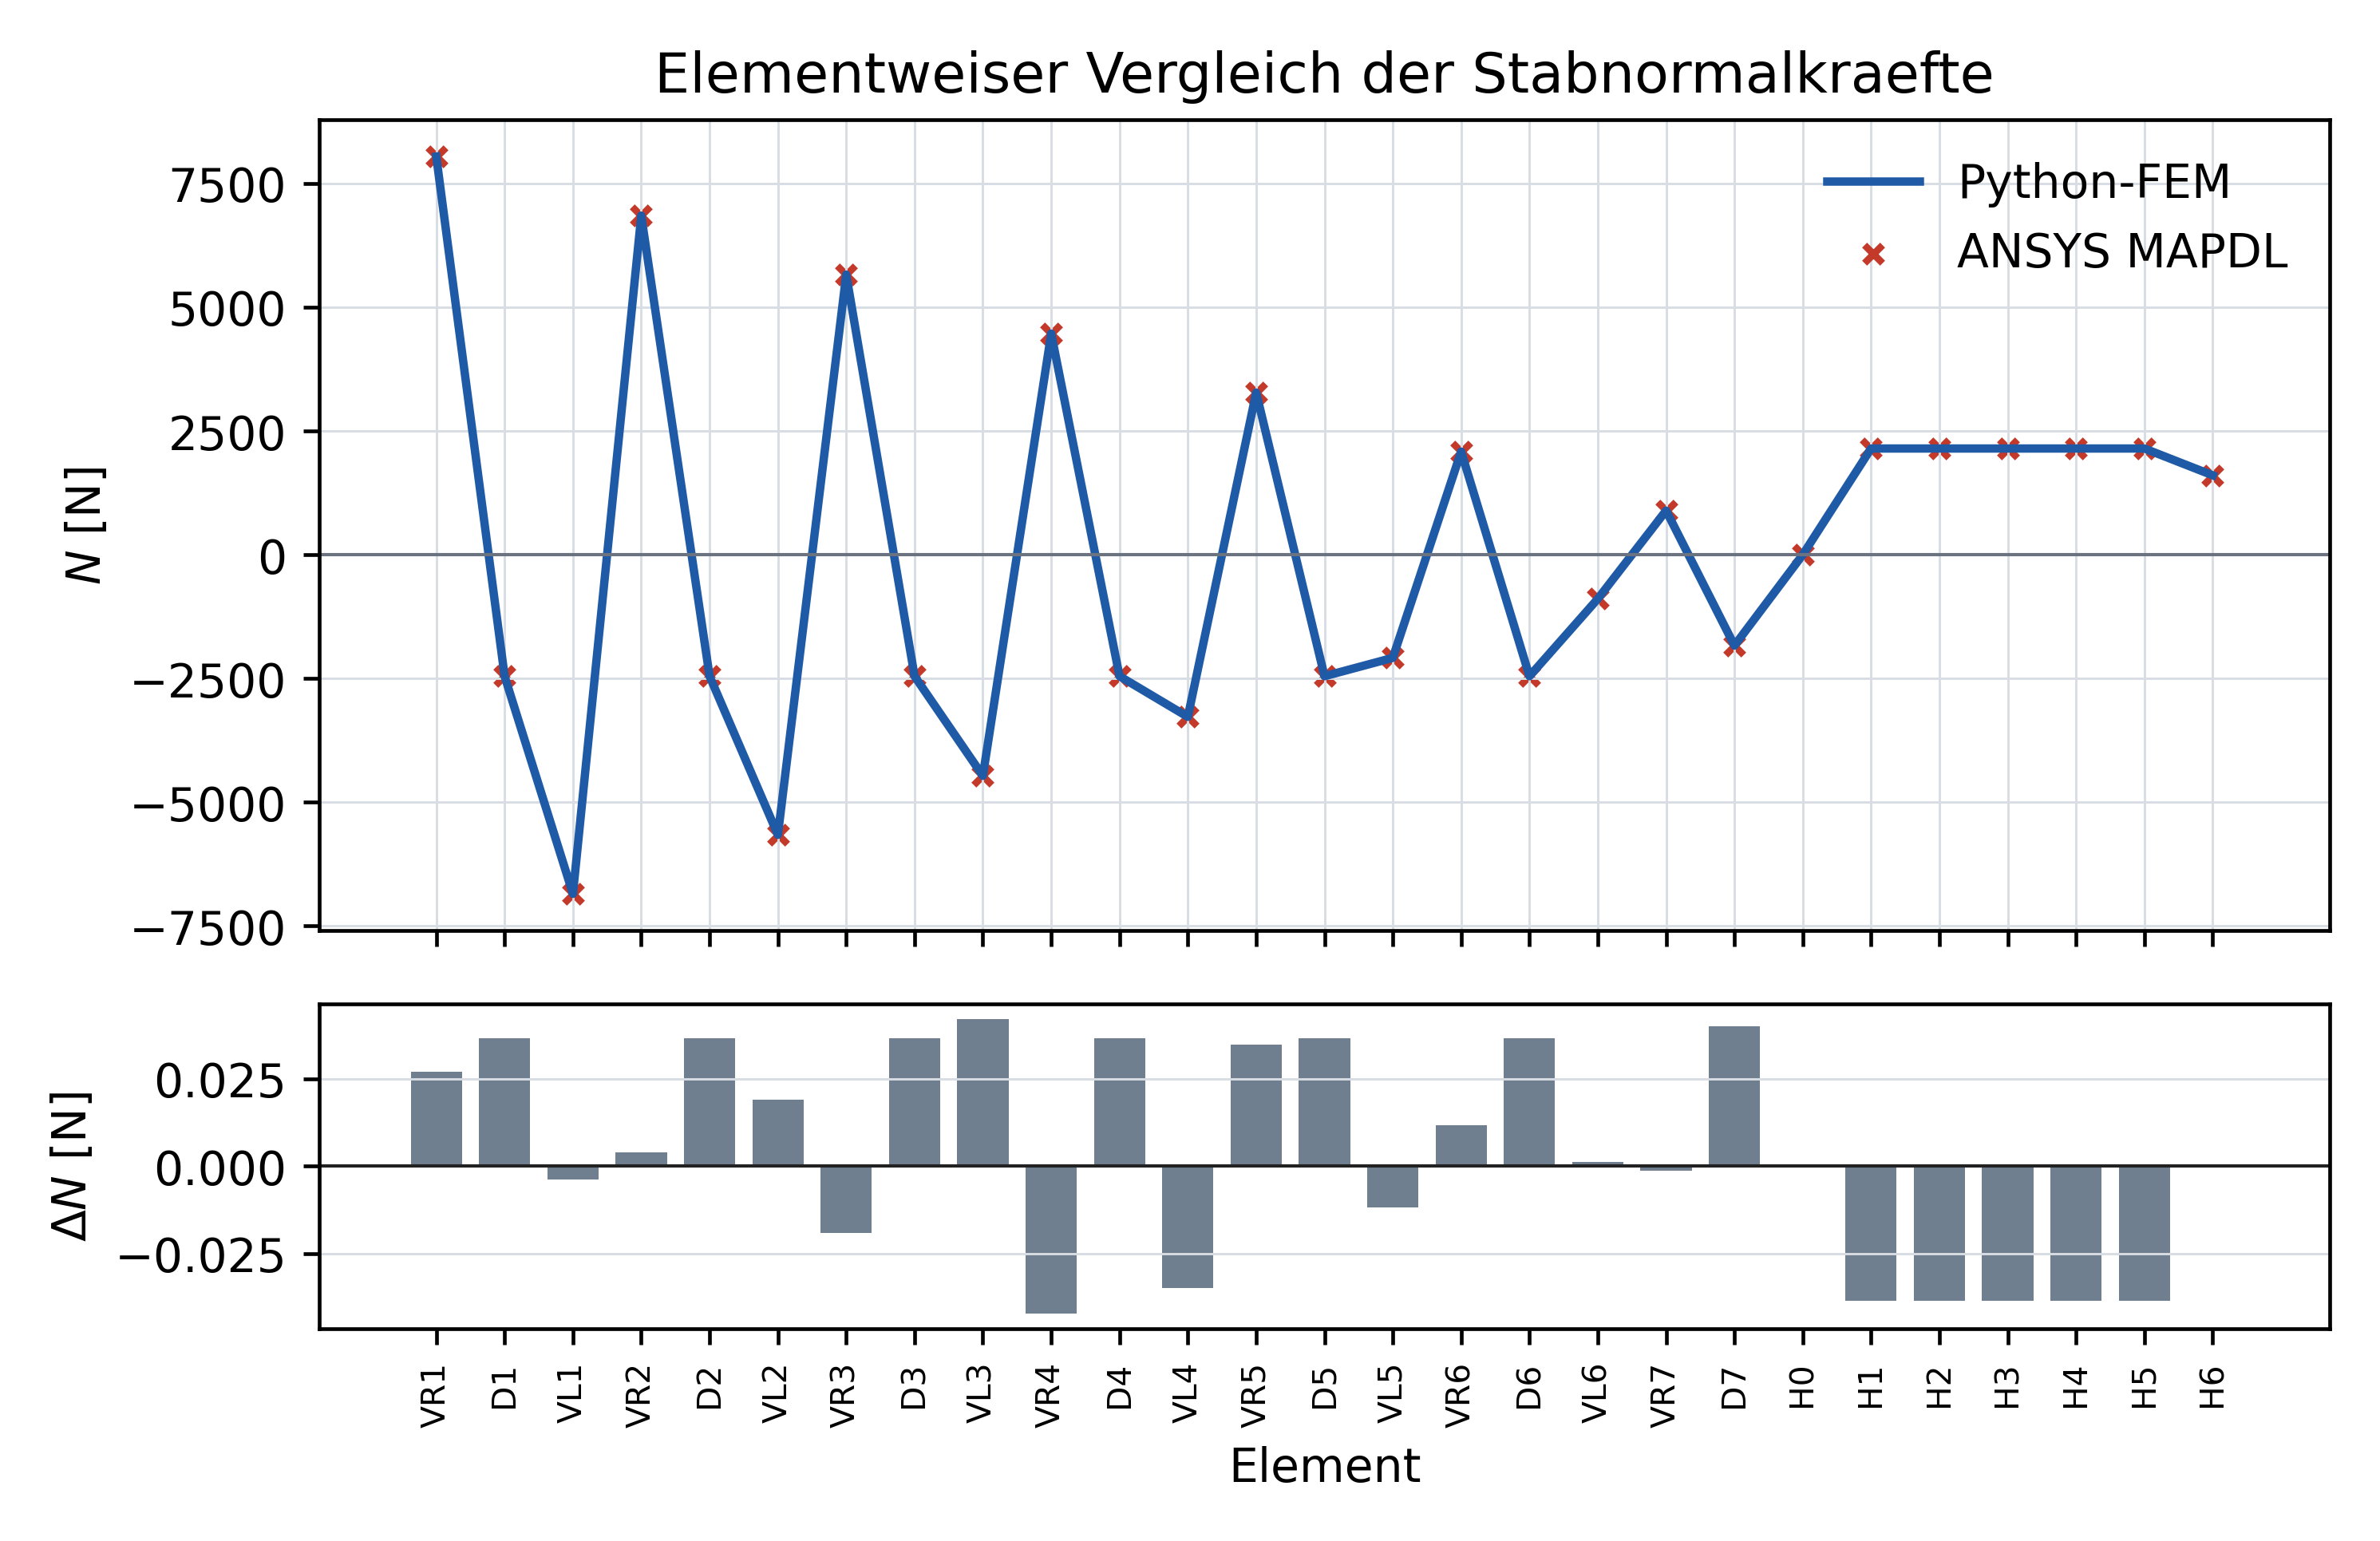
\includegraphics[width=0.92\linewidth]{Aufgabe1/figures/truss_python_ansys_comparison.png}
\caption{Vergleich aller Stabnormalkräfte aus Python-FEM und ANSYS. Oben liegen die ANSYS-Marker auf der Python-Kurve; unten ist die kleine Restabweichung dargestellt.}
\end{figure}

\section{Aufgabe 2: Kerbformzahl einer Scheibe mit Löchern}

\subsection*{2 a) ANSYS-Modell und Konvergenz}
Für Projekt 27 gelten \(d=70\,\mathrm{mm}\), \(\ell=110\,\mathrm{mm}\), \(t=4\,\mathrm{mm}\), \(n_y=10\,\mathrm{N/mm}\). Wegen Periodizität und Symmetrie wurde nur ein symmetrischer Ausschnitt der gelochten Scheibe berechnet. Die Scheibe wurde linear elastisch als ebener Spannungszustand modelliert. Die lokale Netzgröße am Lochrand ist entscheidend, weil dort die maximale Normalspannung \(\sigma_y\) auftritt.

\begin{figure}[H]
\centering
\begin{subfigure}{0.48\linewidth}\centering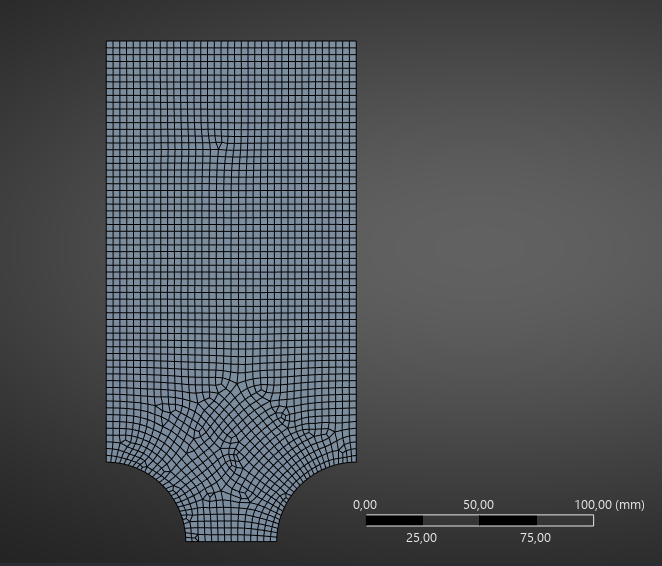
\includegraphics[width=\linewidth,height=0.14\textheight,keepaspectratio]{Aufgabe2/figures/mesh_gesamt_report.png}\caption{Globales Netz}\end{subfigure}
\begin{subfigure}{0.48\linewidth}\centering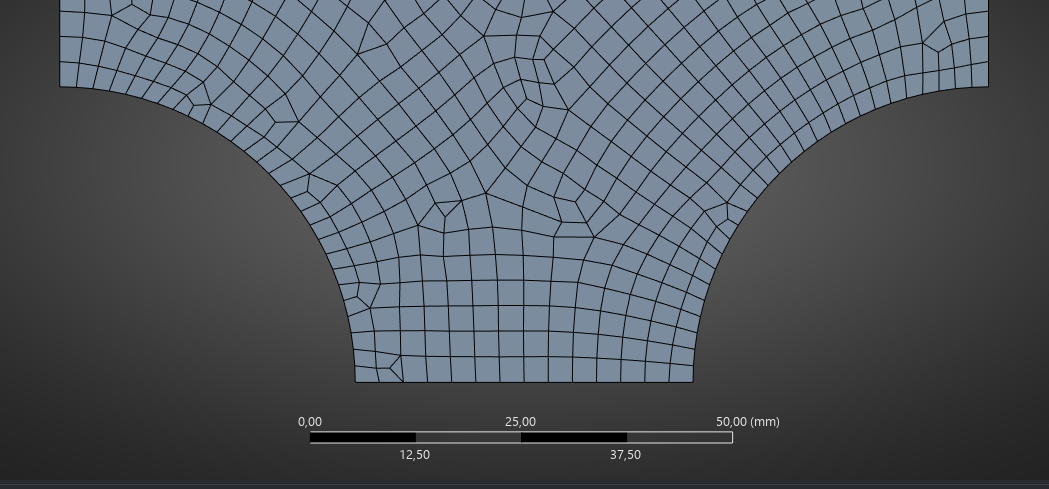
\includegraphics[width=\linewidth,height=0.14\textheight,keepaspectratio]{Aufgabe2/figures/mesh_zoom_report.png}\caption{Lochrandnetz}\end{subfigure}\\[-1mm]
\begin{subfigure}{0.48\linewidth}\centering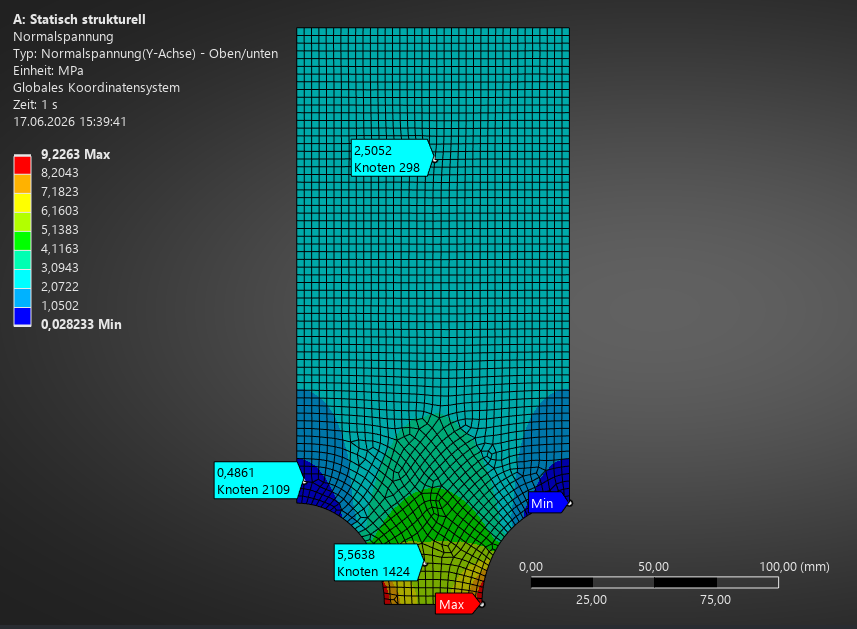
\includegraphics[width=\linewidth,height=0.15\textheight,keepaspectratio]{Aufgabe2/figures/normalspannung_report.png}\caption{\(\sigma_y\)}\end{subfigure}
\begin{subfigure}{0.48\linewidth}\centering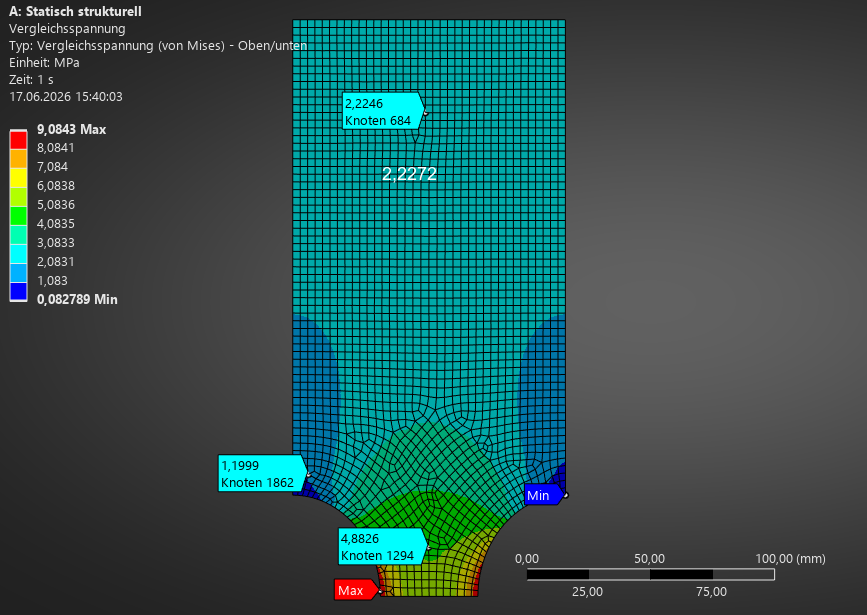
\includegraphics[width=\linewidth,height=0.15\textheight,keepaspectratio]{Aufgabe2/figures/vergleichspannung_mises_report.png}\caption{von Mises}\end{subfigure}
\caption{Aufgabe 2: Netz und Spannungsverteilung, auf den relevanten Modellbereich zugeschnitten.}
\end{figure}

Für \(\alpha_k\) wird nur \(\sigma_y\) ausgewertet; die von-Mises-Spannung dient nur der Darstellung. Die neue Konvergenzreihe wurde aus den ANSYS-Screenshots der lokalen Netzgrößen \(10,8,6,3,2,1\,\mathrm{mm}\) abgelesen.

Die Maximalwerte der Netzstudie für \(\sigma_y\) lauten:
\begin{table}[H]\centering\small
\begin{tabular}{lrrrrrr}
\toprule
lokale Netzgröße [mm] & 10 & 8 & 6 & 3 & 2 & 1\\
\midrule
\(\sigma_{y,\max}\) [MPa] & 9.1539 & 9.2332 & 9.2341 & 9.2157 & 9.2263 & 9.1063\\
\bottomrule
\end{tabular}
\end{table}
Die Maximalspannung ist ein lokaler Knotenwert am Lochrand. Bei feinerer Vernetzung muss dieser Wert nicht streng monoton fallen oder steigen, weil sich die Lage des maximalen Knotens, die Spannungsinterpolation und die Mittelung in ANSYS leicht ändern können. Entscheidend ist deshalb nicht der einzelne letzte Wert, sondern die geringe Schwankung der feinsten Netzstufen. Die Werte für \(3\,\mathrm{mm}\), \(2\,\mathrm{mm}\) und \(1\,\mathrm{mm}\) liegen innerhalb von \(1.31\,\%\); als Referenzwert wird daher deren Mittelwert verwendet.

\begin{figure}[H]
\centering
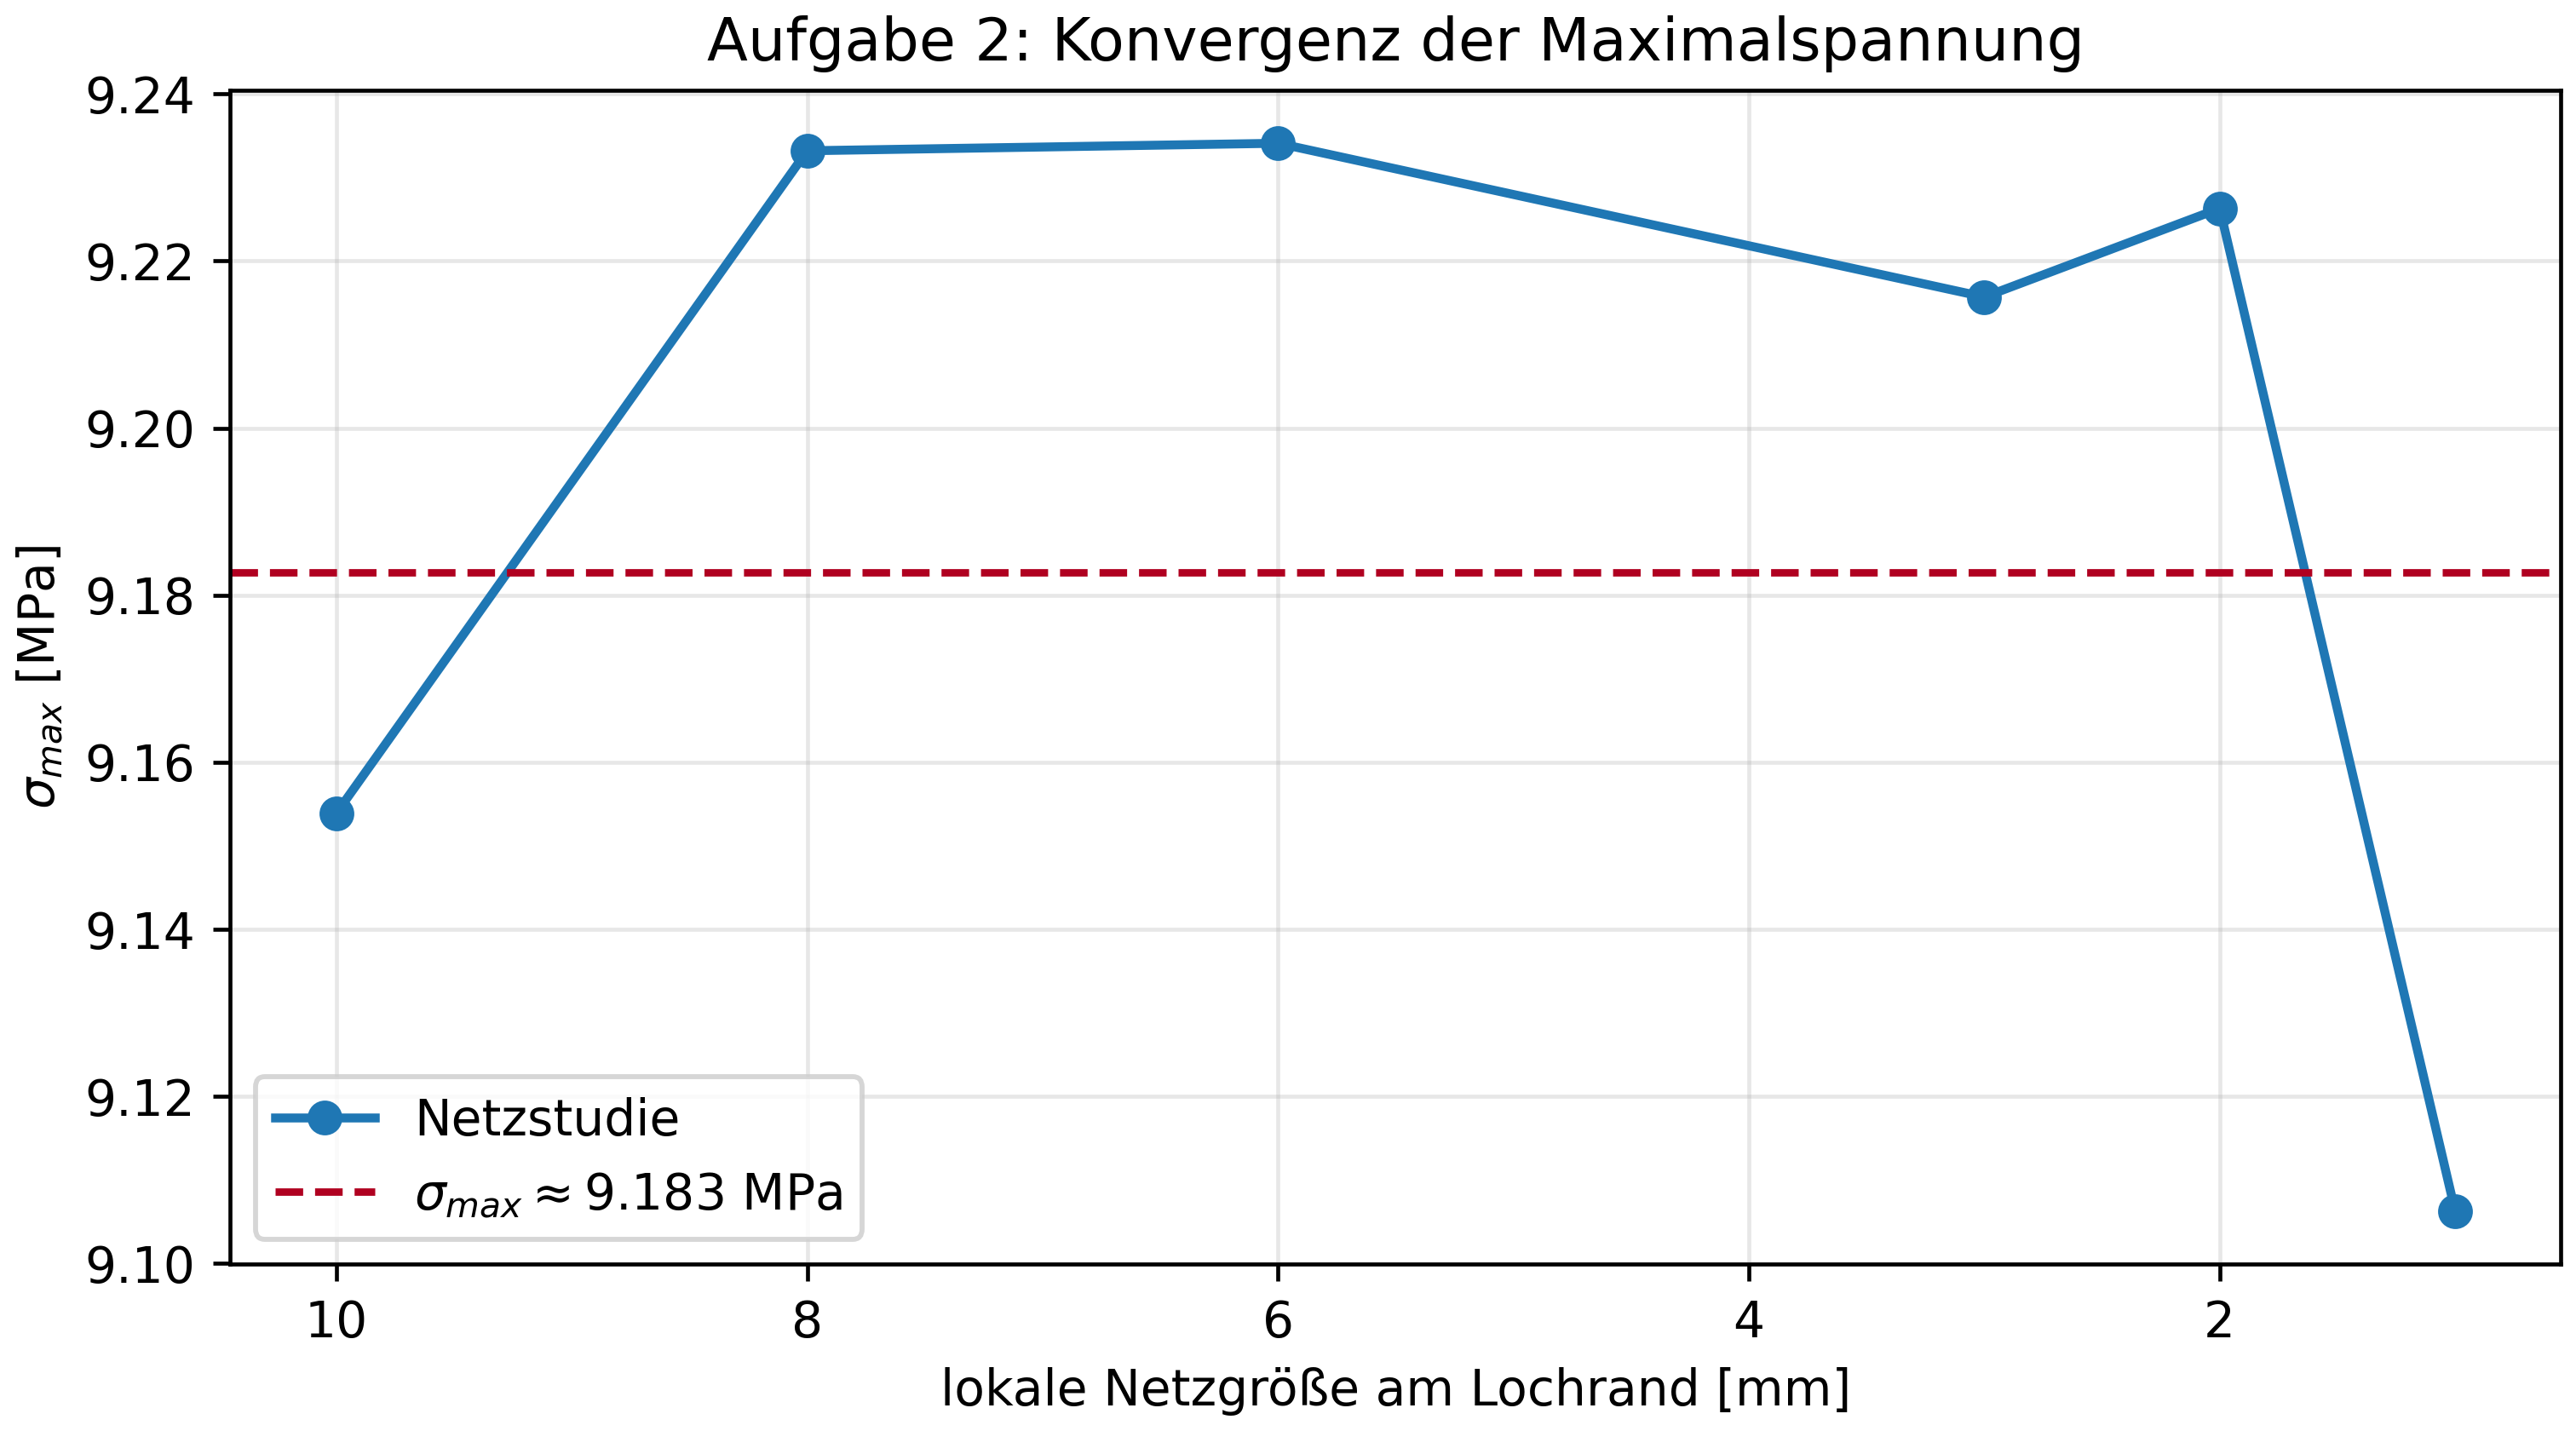
\includegraphics[width=0.62\linewidth]{Aufgabe2/figures/kerb_convergence.png}
\caption{Aufgabe 2: Konvergenz von \(\sigma_{\max}\).}
\end{figure}

\subsection*{2 b)--d) Nennspannung, Kerbformzahl und Ergebnis}
Die Nennspannung ergibt sich aus der Linienlast und der Dicke:
\[
\sigma_n=\frac{n_y}{t}=\frac{10}{4}=2.50\,\mathrm{MPa}.
\]
Mit \(\sigma_{\max}=9.1828\,\mathrm{MPa}\) folgt
\[
\alpha_k=\frac{\sigma_{\max}}{\sigma_n}=\frac{9.1828}{2.50}=3.673.
\]

\begin{table}[H]\centering\small
\begin{tabular}{lr}
\toprule
Größe & Wert\\
\midrule
Nennspannung \(\sigma_n\) & \(2.50\,\mathrm{MPa}\)\\
konvergierte Maximalspannung \(\sigma_{\max}\) & \(9.1828\,\mathrm{MPa}\)\\
Kerbformzahl \(\alpha_k\) & \(3.67\)\\
\bottomrule
\end{tabular}
\end{table}

\section*{Kurzfazit}
Die CFD-Berechnung liefert eine plausible Windlast von \(6430.05\,\mathrm{N}\) mit \(c_D=1{,}874\), passend zur Literaturgrößenordnung quer angeströmter Platten und bestätigt durch den gemittelten Wanddruck. Punktlagerungen der Tafel erzeugen randbedingungsdominierte Spannungsspitzen; die Linienstützen bilden eine realistischere Rückseitenstruktur ab und liefern \(\sigma_v=63.77\,\mathrm{MPa}<\sigma_\mathrm{zul}\): die Tafel ist ausreichend dimensioniert. Träger H3 ist maßgebend; das Fachwerk und die Python-Nachrechnung sind mit den gewählten Rohrquerschnitten ausreichend dimensioniert und stimmen mit ANSYS überein. Für Aufgabe 2 ergibt sich \(\alpha_k=3.67\).

\end{document}
